\documentclass[12pt,twoside]{article}
%\documentclass[a4paper,10pt,twoside]{article}
\usepackage{ucs}
\usepackage[utf8x]{inputenc}
\usepackage[english,hebrew]{babel}
\usepackage{culmus}
%\usepackage{culmus}

%\usepackage{float}
%\usepackage{listings}
\usepackage{color} %red, green, blue, yellow, cyan, magenta, black, white
\definecolor{mygreen}{RGB}{28,172,0} % color values Red, Green, Blue
\definecolor{mylilas}{RGB}{170,55,241}


%\usepackage{xkeyval}
\usepackage{graphicx}

\usepackage{epstopdf}
%\usepackage{eucal}
%\usepackage{mathrsfs}
%\usepackage{theorem}
%\usepackage{pifont}
\usepackage{epsfig}
%\usepackage[colorlinks=true, bookmarks=true]{hyperref}
\usepackage{bibtopic,wrapfig}
%\usepackage{bbding}
%\usepackage{fancyhdr}
%\usepackage{verbatim}

%\pagestyle{fancy}

%\usepackage{bidi}


%\rhead{\thepage}
%\lfoot{\small \copyright\;\;\; שירה בר-דב, אורט בראודה}
%\rfoot{\thepage}
%\cfoot{}
%\renewcommand{\headrulewidth}{0.4pt}
%\renewcommand{\footrulewidth}{0.4pt}
%\DeclareGraphicsExtensions{.pdf,.png,.jpg}
%\let\arref\ref
%\renewcommand{\ref}[1]{\I{\arref{#1}}}

% User packages
%%%%%%%%%%%%%%%%%%%%%%%%%%%%%%%%
\usepackage{subcaption}
\usepackage{mathtools}
\usepackage{pdfpages}


%\rhead{\thepage}
%\lfoot{\small \copyright\;\;\; שירה בר-דב, אורט בראודה}
%\rfoot{\thepage}
%\cfoot{}
%\renewcommand{\headrulewidth}{0.4pt}
%\renewcommand{\footrulewidth}{0.4pt}
%\DeclareGraphicsExtensions{.pdf,.png,.jpg}
%\let\arref\ref
%\renewcommand{\ref}[1]{\I{\arref{#1}}}

\setlength{\parskip}{6pt} \setlength{\parindent}{0pt}
\setlength{\oddsidemargin}{0pt} \setlength{\evensidemargin}{0pt}

% User defined macros
%%%%%%%%%%%%%%%%%%%%%%%%%%%%%%%%

\newtheorem{definition}{הגדרה}[section]
\newtheorem{theorem}{משפט}[section]
\newtheorem{proposition}{טענה}[section]
\newtheorem{conjecture}{השערה}[section]
\newtheorem{corollary}{מסקנה}[section]
\newtheorem{lemma}{למה}[section]
\newtheorem{example}{דוגמה}[section]
\newtheorem{comm}{הערה}[section]

\newcommand{\sumi}[1]{\sum_{#1=1}^n}
\newcommand{\Zn}{{Z_2}^n}

%\numberwithin{equation}{section}

%\documentclass{amsart}
%%\usepackage[active]{srcltx} % SRC Specials for DVI Searching
%\usepackage {epsfig}
%% THEOREM Environments ---------------------------------------------------
% \newtheorem{thm}{Theorem}
% \newtheorem{cor}[thm]{Corollary}
% \newtheorem{lemma}[thm]{Lemma}
% \newtheorem{prop}[thm]{Proposition}
% \newtheorem{theorem}[thm]{Theorem}
% \theoremstyle{definition}
% \newtheorem{defn}[thm]{Definition}
% \theoremstyle{remark}
% \newtheorem{rem}[thm]{Remark}
%% MATH -------------------------------------------------------------------
%%%% ----------------------------------------------------------------------
%\setlength{\textheight}{43pc} \setlength{\textwidth}{28pc}
%

% User defined macros
%%%%%%%%%%%%%%%%%%%%%%%%%%%%%%%%


\begin{document}

\begin{titlepage}
\newcommand{\HRule}{\rule{\linewidth}{0.5mm}} % Defines a new command for the horizontal lines, change thickness here

\center % Center everything on the page

%----------------------------------------------------------------------------------------
%   HEADING SECTIONS
%----------------------------------------------------------------------------------------

\textsc{\LARGE   
% מכללת אורט בראודה
% Name of your university/college
}\\[1.5cm]
\textsc{\LARGE 
המחלקה למתמטיקה שימושית
 % Major heading such as course name
}\\[0.5cm]

%----------------------------------------------------------------------------------------
%   TITLE SECTION
%----------------------------------------------------------------------------------------

\HRule \\[0.4cm]
{ \huge \bfseries
חקירת משחק האורות
% Title of your document
 } \\[0.4cm] 
\HRule \\[1.5cm]

%----------------------------------------------------------------------------------------
%   AUTHOR SECTION
%----------------------------------------------------------------------------------------

\begin{minipage}{0.4\textwidth}
\begin{flushleft} \large
\emph{מאת:}\\
ולדיסלב ברקנס
% Your name
\end{flushleft}
\end{minipage}
~
\begin{minipage}{0.4\textwidth}
\begin{flushright} \large
\emph{מנחה:} \\
אלכס גולוורד 
% Supervisor's Name
\end{flushright}
\end{minipage}\\[2cm]
%----------------------------------------------------------------------------------------
%   DATE SECTION
%----------------------------------------------------------------------------------------

{\large \today}\\[2cm] % Date, change the \today to a set date if you want to be precise
%----------------------------------------------------------------------------------------
%   LOGO SECTION
%----------------------------------------------------------------------------------------
\begin{figure}
	\begin{center}
		\L{\includegraphics[scale=0.3]{images/Braude_Logo.jpg}}
	\end{center}
%	\caption{הפונקציה $\arctan(x)$ - באדום, וסכום שלושת האיברים הראשונים של טור טיילור שלה - בכחול}
%	\label{atan}
\end{figure}

%\includegraphics[scale=0.3]{Braude_Logo}\\[1cm] % Include a department/university logo - this will require the graphics package
%----------------------------------------------------------------------------------------

\vfill % Fill the rest of the page with whitespace

\end{titlepage}
%----------------------------------------------------------------------------------------
%   תוכן עניינים
%----------------------------------------------------------------------------------------
\tableofcontents

\newpage
%--------------------------------------------------------------------------------------
%   הקדמה
%----------------------------------------------------------------------------------------
\section{הקדמה}
עבודה זה הינה עבדות סוף של סטודנט במחלקה למתמטיקה שימושית.
עבודה זה 
מבוססת על משחק האורות 
ונבנתה 
על  גבי שאלות ששאלנו את עצמנו במהלך חקירת המשחק.
חיפוש פתרונות הוביל למחקר ותוצאות מעניינות 
שלא ברורות מעליהן.

השאלות לדוגמה שעלו בעבודה הן שיטות למציאת פתרון למשחק.
מצאנו שתי שיטות, שבדיעבד נראו כשונות אבל הצלחנו להראות את הקשר בשתי השיטות.
בנוסף 
לאחר שהיה לנו אלגוריתם שפותר את המשחק שמנו לב שאם מתחילים את המשחק 
במצב התחלתי מוכר לכל משחק שכזה קיים לפחות פתרון אחד,
תופעה שכזה גרמה לנו לחפש ולמצוא הוכחה למה באמת קיים לפחות פתרון אחד במצבים התחלתיים עלו.
דבר אחרון שעסקנו בו הוא בחיפוש סוג מסוים של פתרונות, פתרונות מינמלי שנגדיר בעבודה. 
סוג הפתרונות שכזה כל כך לא נפוץ שהצלחנו להוכיח את כל המקרים 
בהם אתכן פתרון שכזה.

עבודה בשבילי הייתה מהנה אני מודה למחלקה 
למתמטיקה שימושית ובמיוחד לאלכס גולדוואסר על הזדמנות לעשות 
עבודה מרתקת שכזה.

תודה רבה

\newpage

\section{רקע על משחק האורות}
משחק האורות או 
\L{Lights Out}
בלועזית,
זהו משחק בו יש לוח משבצות ריבועי.
כל משבצת הינה לחצן על הלוח שיכולה להיות בשתי מצבים
דלוק או כבוי.
כאשר לוחצים על משבצת, משבצת הנלחצת וכל משבצות הסמוכות לה כלומר,
כל המשבצת בעל צלע משותפת משנות את מצב נוכחי.

משחק במקור נימכר כאשר המצב התחלתי של הלוח כולו עם משבצות דלוקות והמטרה לכבות את כל המשבצות על הלוח כולו.
קיימים גם משחקים שמצב התחלתי הוא אקראי ומנסים לכבות או להדליק את כל המשבצות.

נתאר זאת ויזואלית: 

\begin{figure}[ht]
    \begin{subfigure}{.5\textwidth}
        \unsethebrew
        \caption{\R{מצב התחלתי}}
        \centering
        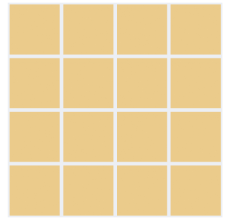
\includegraphics{images/4x4_start_board.PNG}
        \sethebrew
    \end{subfigure}%
    \begin{subfigure}{.5\textwidth}
        \unsethebrew
        \caption{\R{לחיצה על משבצת מסומנת}}
        \centering
        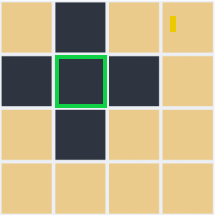
\includegraphics{images/4x4_press.PNG}
        \sethebrew
    \end{subfigure}%
\end{figure}

נבחין כי המשחק 
$4 \times 4$
מתחיל במצב
\L{(a)}.
בלוח 
\L{(b)}
נתאר מצב בו לחצו על משבצת המסומנת, בירוק
כל המשבצות השכנות והיא משנות מצבן, היות ומצב של כולן היה דלוקות לכן הן נכבו

המשחק במקור היה צעצוע אלקטרוני על לוח 
$5 \times 5$
ששוחרר ב 
$1995$.
המשחק יכול להראות פשוט אבל כפי שתואר
במאמר
\cite{B1}
כ
\L{"devilish invention"}.
קיים קושי רב בלמצוא שיטה לפתרון אינטואיטיבי.
בנוסף אציין מניסיון האישי שהמשחק קשה כבר 
על לוח 
$5 \times 5$
ולרוב אנשים שמשחקים אותו מכירים מצבים על הלוח שיודע להם פתרון ומנסים להגיע למצבים עלו.

פרויקט זה באה בעקבות הקושי של המשחק
והניסוי להציע שיטות לפתרון, בעקבות ניסיונות עלו
נעזרנו במספר רב של כלים מתמטיים מתקדמים.

קיימים המון שאלות שקשורות למשחק וננסה בפרויקט זה להציג פתרון לחלקם.
חוץ מאתגר של המשחק עצמו קיים אתגר מתמטי שנרצה בפרויקט זה להציג.

\subsection{ משחק האורות על גרף}
אחרי שכללי המשחק על לוח הובנו אפשר לנסות להכליל את המשחק כמשחק על גרף.
קיימים הרבה סיבות בהם תירצה להגדיר את הבעיה על מבנה כללי שכזה:

\begin{enumerate}
    \item 
    ככול שמבנה כללי יותר תאוריה שאתה מפתח מתאימה ליותר בעיות.
    \item 
    קיימת תאוריה רחבה שפותחה על גרפים ואתכן שנעזר בה.
    \item 
    מבליט את מהות הבעיה והגדרה הבסיסית ביותר של המשחק.
\end{enumerate}

ארצה להתייחס לנקודה אחרונה, זה שאפשר לתאר את הבעיה של משחק
כאוסף של כללים על גרף, מרכזת אותנו לבעיה ובסופו של דבר כשנראה את שיטה למציאת
הפתרון, השיטה עצמה תזכיר לנו מיד את שיטה לייצוג הגרפים בעזרת מטריצה.

כדי לתאר את משחק האורות על גרף נשתמש באותם כללים שהגדרנו פרט לעובדה
שצמתים הם הלחצנים שבמקרה של הלוח היו המשבצות
ונזכיר שכל לחיצה על צומת הופכת את המצב של הצומת והשכנים שלה.
נזכיר כי צמתים שכנים הם צמתים שיש
קשת ביניהם.

נציין כי כאשר כל צומת יכולה להיות בשתי מצבים,
דלוקה או כבויה המטרה היא לעבור מכל הצמתים במצב מסוים דלוק למצב אחר כבוי.

העובדה שמצב התחלתי הינו דלוק או כבוי אינה תשנה את המשחק עלה רק לאיזה מצב סופי צריך לעבור
לכבוי או דלוק.

\begin{figure}[ht]
    \caption{\R{משחק על גרף לדוגמה}}
    \label{fig: start game in graph}
    \begin{subfigure}{.5\textwidth}
        \unsethebrew
        \caption{\R{מצב התחלתי}}
        \centering
        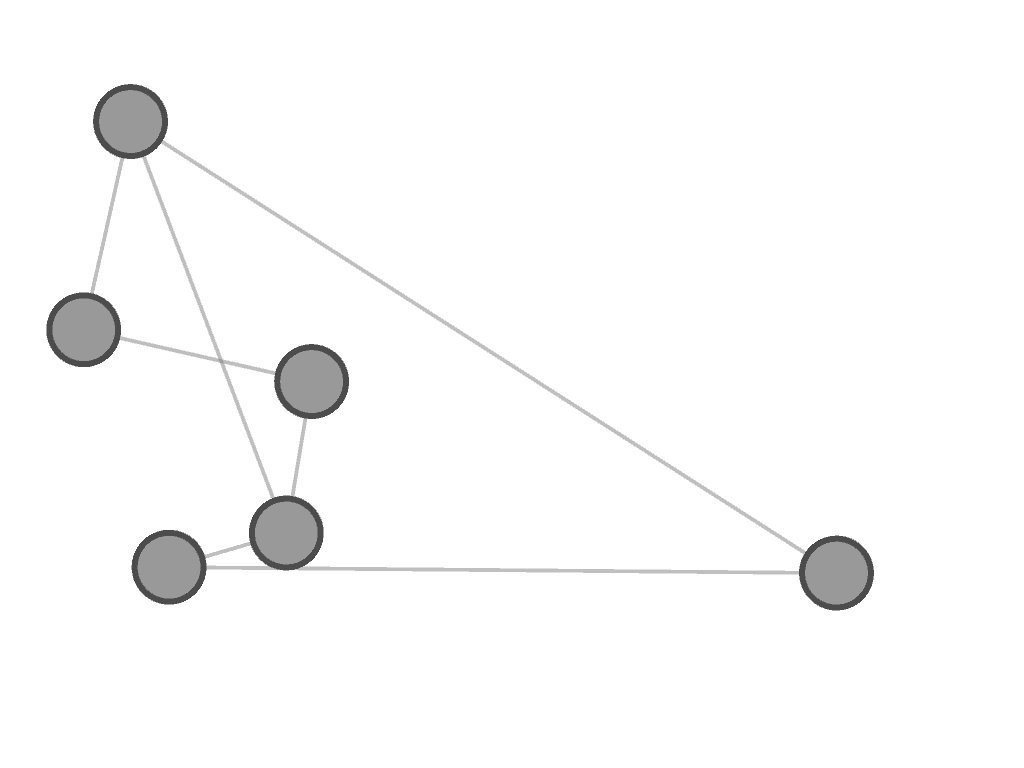
\includegraphics[width=\textwidth,height=\textheight,keepaspectratio]{images/graph_start_board.png}
        \sethebrew
    \end{subfigure}%
    \begin{subfigure}{.5\textwidth}
        \unsethebrew
        \caption{\R{לחיצה על משבצת מסומנת}}
        \centering
        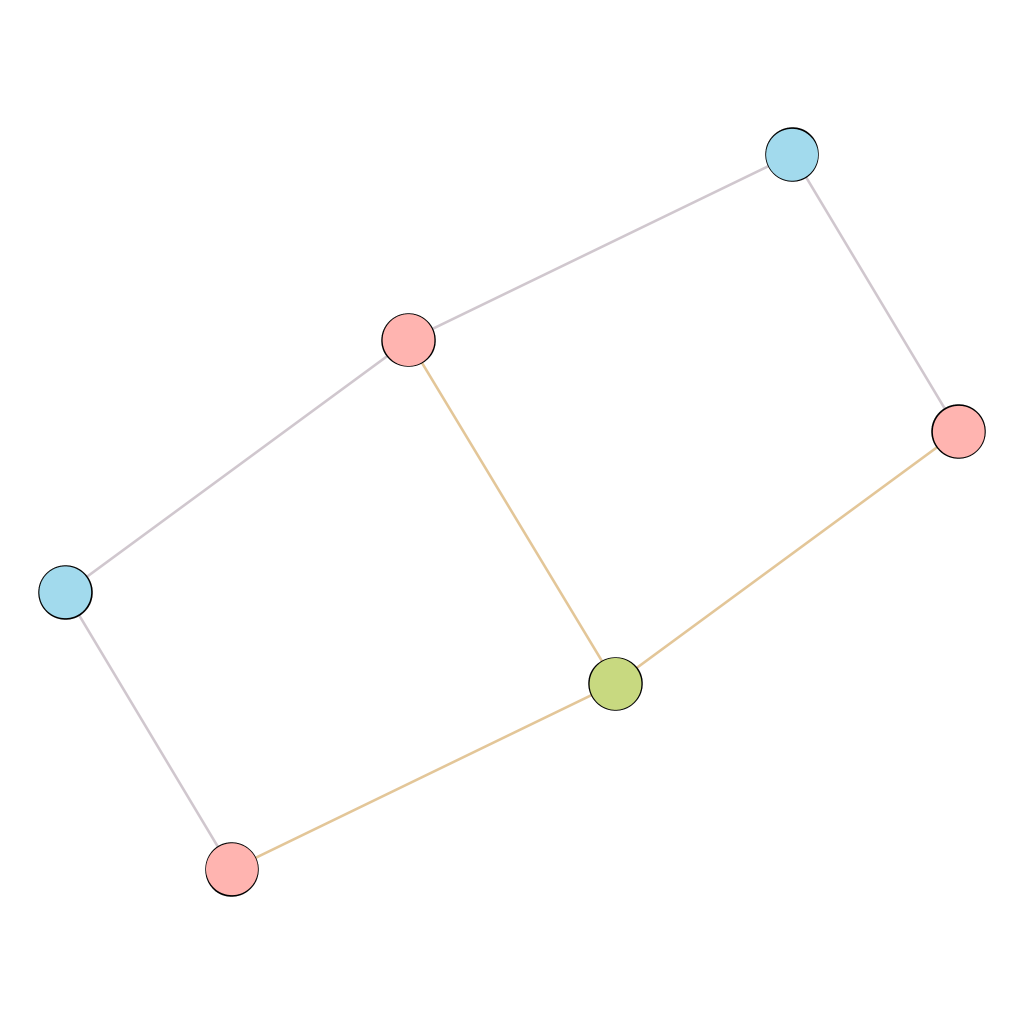
\includegraphics[width=\textwidth,height=\textheight,keepaspectratio]{images/graph_press.png}
        \sethebrew
    \end{subfigure}%
\end{figure}

נמחיש זאת על דוגמה שבאיור
\ref{fig: start game in graph}
כאשר הגרף התחלתי
\L{(a)}
ניתן לראות
$6$
קודקודיים
צבועים באפור כלומר כבויים ומטרה של המשחק להדליק את כל הצמתים כלומר לצבוע את כולם בצהוב.

בשלב 
\L{(b)}
מציגים  לחיצה על צומת ירוקה היא ושכניה נצבעים בצהוב.

\begin{comm}
    בפועל צומת ירוקה גם נצבעת לצהוב צביעה לירוק נועדה להדגשה על מי בוצע הלחיצה
\end{comm}

משחק על גרף הינה הכללה  של משחק על לוח כלומר, כל משחק 
לוח ניתן לתאר בעזרת משחק על גרף.

נמחיש זאת על דוגמה, ניקח לוח למשל
$2 \times 3$
נמספר את המשבצות כמו באיור
\ref{2x3_board}

כדי לתאר את הלוח על על משחק גרף נשתמש בשני הכללים הבאים:
\begin{enumerate}
    \item 
    כל משבצת על משחק לוח נהפוך לצומת.
    \item 
    כל זוג משבצות סמוכות על לוח נחבר את הצמתים בצלע
\end{enumerate}

\begin{figure}[ht]
    \caption{
        \R{לוח
        $2 \times 3$
        }
    }
    \label{2x3_board}
    \unsethebrew
    \centering
    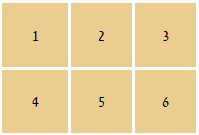
\includegraphics[width=0.5\textwidth,height=0.5\textheight,keepaspectratio]{images/2x3_board.PNG}
    \sethebrew
\end{figure}

הגרף שנקבל עבור לוח באיור
\ref{2x3_board}
מתואר באיור
\ref{2x3_graph}

\begin{figure}[ht]
    \caption{
        \R{גרף
        $2 \times 3$
        }
    }
    \unsethebrew
    \centering
    \label{2x3_graph}
    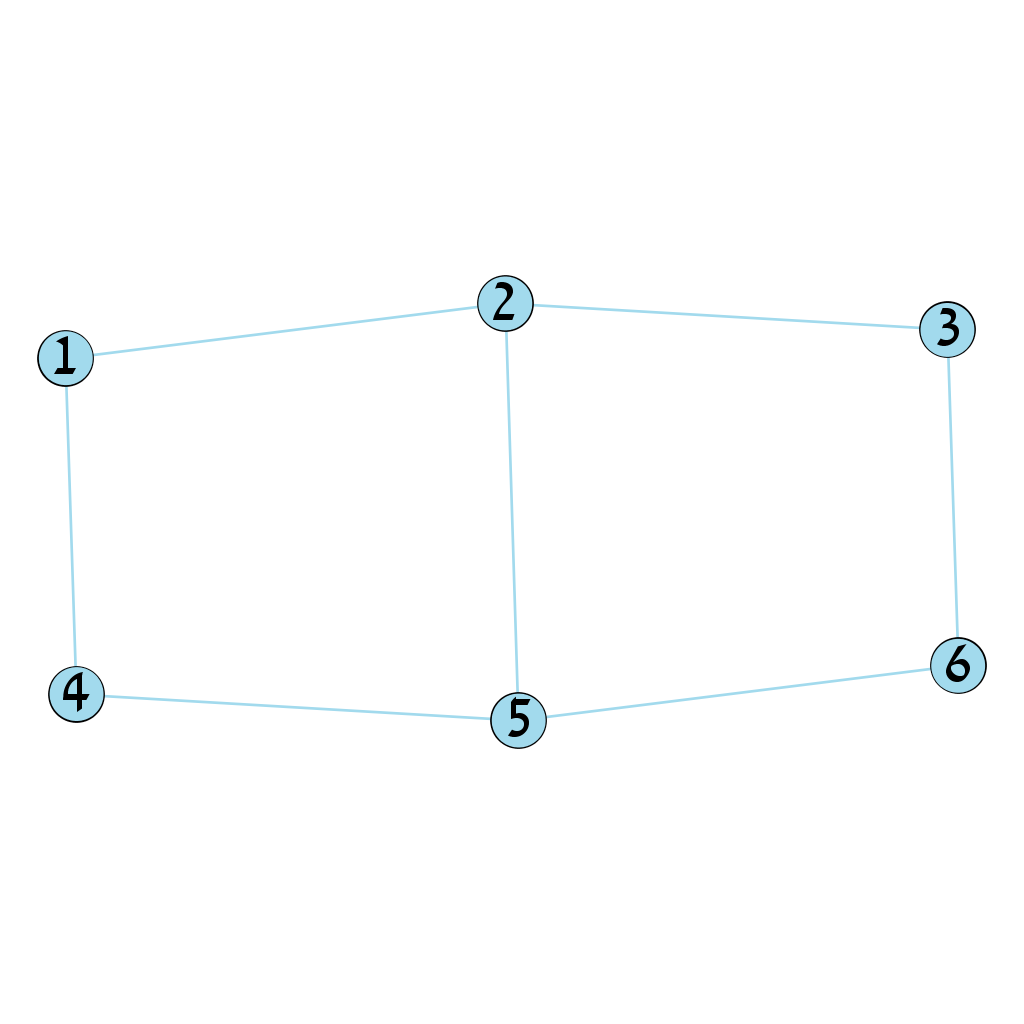
\includegraphics[width=0.5\textwidth,height=0.5\textheight,keepaspectratio]{images/2x3_graph.png}
    \sethebrew
\end{figure}

\begin{comm}
    קיימים הרבה משחקים שמתוארים על גרף אבל לא ניתן לתאר אותם על לוח
    לדוגמה,
    גרף בו יש צומת אם יותר מ
    $4$
    שכנים לא ניתן לתאר לוח שכזה כיוון שלכל משבצת על לוח
    יש לכל יותר 
    $4$
    משבצות סמוכות.
\end{comm}

\begin{comm}
    בעזרת שיטה שתיארנו אפשר להפוך כל משחק לוח למשחק על גרף, אבל להפך הוא לא נכון 
    כלומר לא כל משחק על גרף אפשר להפוך למשחק על לוח.
\end{comm}

בגלל שכל משחק לוח ניתן לתאר אותו כמשחק על גרף לכן המשפטים המרכזיים ננסה לנסח על משחקים על גרף כי אז הם היו נכונים
גם על משחקים על לוח.


\newpage

\section{ אלגוריתם למציאת פתרון}
לפני שנציג את שיטות למציאת פתרון, נשאל את עצמנו מדוע בכלל צריך למצוא שיטות עלו.
הרי בסופו של דבר זה משחק ולהציע פתרון למשחק יפגע במהותו משחק הרי אף אחד לא ירצה
לשחק במשהו שידוע מה הפתרון שלו.

הצורך למצוא פתרון הוא נוראה טבעי וזה בעקבות שמשחק עצמו מעניין.
אם תנסה לשחק במשחק פתיר על לוח התחלתי כלשהו לא בהכרח המצב התחלתי שבו כל הנורות דלוקות או כבויות
על לוח 
$3 \times 3$
המשחק ניראה תמים ופשוט אתה מתחיל לצפות לאיזושהי חוקיות.
\\
בשלב הזה שאתה כבר מנסה לוח 
$4 \times 4$
המשחק מתגלה כלא פשוט כשאתה מנסה לוח בקונפיגורציה כלשהי לא בהכרח התחלתית
מהר מאד אתה נעבד.
\\
בשלב מסוים גם לוח 
$4 \times 4$
נהיה מוכר ובאופן תמים תנסה לעבור ללוח
$5 \times 5$
ומהר מאד הלוח שובר את רוחה.
קיימים כל כך הרבה מכירים שנשארת לך משבצת אחת שנותרה לסדר ואינה נעלמת
האינטואיציה שחשבת שפיתח על לוח 
$4 \times 4$
נעלמת כאילו למדת לשחק משחק חדש 
כשעברת לשחק למשחק
על לוח
$5 \times 5$.

התופעה הזאת ששינוי גודל מרגיש שהתחלת משחק אחר עוד
מורגשת בשלב שאתה מנסה לפתור את מצב התחלה בלוחות שונים

\begin{figure}[ht]
    \caption{\R{פתרונות של משחק על לוחות שונים}}
    \unsethebrew
    \label{fig:sol_3_4_5}
    \centering
    \begin{subfigure}[b]{.25\linewidth}
    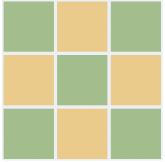
\includegraphics[width=\linewidth]{images/3x3_sol.PNG}
    \end{subfigure}
    \begin{subfigure}[b]{.25\linewidth}
    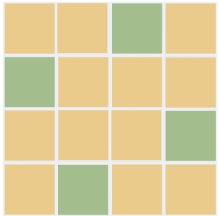
\includegraphics[width=\linewidth]{images/4x4_sol.PNG}
    \end{subfigure}
    \begin{subfigure}[b]{.25\linewidth}
    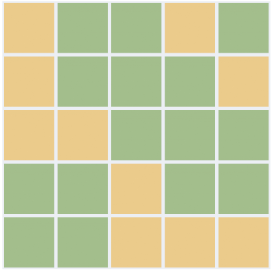
\includegraphics[width=\linewidth]{images/5x5_sol.PNG}
    \end{subfigure}

\end{figure}
\sethebrew

איור
\ref{fig:sol_3_4_5}
באה להמחיש את חוסר  אינטואיציה
כאשר האיור מתאר את פתרון כלשהן של משחק על הלוח כאשר הלוח במצב התחלתי בו כל נורות דלוקות.
כדי שהשחקן ינצח עליו ללחוץ על המשבצות הירוקות.
\\
איור באה להראות שלוחות על קטנים מ
$5 \times 5$
אתכן ותחשוב שפתרון נוצר על לחיצות סימטריות והאיור ממשיך שזה לא כך 
כי כאשר מסתכלים על הלוח 
$5 \times 5$
מיד אפשר לראות שפתרון לא ניראה סימטרי.

חוסר האינטואיציה מתבלט גם מהעבודה שכמות הפתרונות משתנה לכל לוח.
עבור לוח 
$3 \times 3$
קיים פתרון יחיד,
אבל ללוח 
$4 \times 4$
קיים
$16$
פתרונות.
כמה פתרונות היה ללוח
$5 \times 5$
,
האם זה יותר או פחות מלוח
$4 \times 4$
בהפתעה רבה ללוח 
$5 \times 5$
יש רק 
$4$
פתרונות זה עובדה מפתיע כי אפשר היה לצפות שמספר פתרונות על לוח גדול יותר אגדל.

אפשר להוסיף שעבור לוחות ריבועים כלומר
$n \times n$
כמות הפתרונות כל כך לא צפויה כי עברו 
$n \in [1,20]$
מספר הפתרונות הגדול ביותר הוא ללוח
$n = 19$ 
ומספר פתרונות 
$65536$.
$n = 19$ 
 יחיד ב
$n \in [1,20]$
שכמות הפתרונות שכזה.

מספר הפתרונות השני הגדול ביות הוא רק
$256$.
ומתקיים ל
$n \in \{9, 16 \}$.

חוץ מבעיית חוסר אינטואיציה לחיפוש פתרון טבעי אפשרי לנסות
פתרון נאיבי המנסה כל לחיצה.
\\
פתרון הנאיבי נפסל ברגע הזה שחושבים על כמה קומבינציות לחיצה קיימות.

\begin{lemma}
    כמות האפשרויות לחיצה על לוח
    $m \times n$
    הוא 
    $2^{m \cdot n}$
\end{lemma}
נומר שאפשרויות לחיצה זה חסם על כמות המצבים האפשריים שמשחק יוכל להיות.
חסימה זאת נובעת משאלה אם שחקן לוחץ על לחצן כמה יכול להשפיע על הלוח.
מובן שאם שחקן לחץ על לחצן מספר זוגי של פעמיים המצב יחזור למצב שהיה.
לכן,
כל לחצן משפיע על הלוח אם הוא נלחץ או לא כלומר, יכול להיות בשתי מצבים.
היות וללוח
$m \times n$
קיים 
$m \cdot n$
לחצנים
,
היות וכל לחצן 
יכול להיות בשתי מצבים שונים
לכן נקבל 
שמספר אפשרויות לחיצה 
ללחצן 
$2$
ול
$m \times n$
לחצנים
$2^{m \cdot n}$.

כבר בלוח 
$6x6$
כמות  אפשרויות לחיצה גדולה 
מכמות הסטנדרטית שמציגים מספר שלמים,
4 בתים או 
$2^{32}$
מספרים,
המטרה של המחשה זה להדגיש כמה לא פרקטית אופציית הפתרון שכזה.

עכשיו שיש לנו מוטיבציה למצוא פתרון השאלה היא באיזה כלים נשתמש, שיטות למציאת פתרון היו מבוססות
מידול מתמטי לבעיה על שדה לינארי ותיאורה כמערכת משוואות, תיאור הבעיה
כמערכת משוואת לינארית תעזור לנו אחר כך לתאר תופעות נוספות כמו מספר פתרונות שונים
שיש לבעיה.

אתכן ויש כמה דרכים להגיע לאותה מודל לינארי שנציע, נציג בעובדה זה שני דרכים אחת 
בעזרת וקטורי שינוי שנתאר בהמשך אותם ומניסיון למצוא צירוף לינארי של וקטורים עלו נמצא את פתרון, דרך שניה תהיה
לפי מערכת משוואות שמתארת את בעיה  בצורה קצת לא מובנת.

היופי זה שאפשר להראות ששתי השיטות מובילות לאותה מערכת משוואות
ונפתור את המשחק בעזרת חיפוש פתרון של המערכת.

בחרנו להציג קודם בעזרת וקטורי שינוי משום שהגדרת וקטורים פשוטה יותר להסבר לאחר שניראה את הדרך הראשונה
הדרך השנייה קלה תהיה יותר מובנת.

כדי למדל את הבעיה על שדה לינארי נזכר בייצוג גרפי שאומר כי לחיצה על צומת משנה את הצומת ושכניה 
אם נסמן את צמתים ב
$n_i$
אז אפשר לתאר כי המצב אתחלתי של משחק על גרף הוא שכל צומת אם הערך התחלתי
$n_i = 0$
וכל צומת יכול לקבל 2 ערכים שנסמן אותם ב
${0,1}$
כאשר 
$0$
מצב התחלתי שכל צמתים התחילו 
ו
$1$
מצב סופי של משחק 
המשחק מסתיים כשכל הצמתים מקיימים
$n_i = 1$.
אנחנו עובדים על שדה בינארי
שנסמן
$Z_2$.

\begin{definition}
    תהי 
    משחק על גרף בעל
    $n$
    צמתים
    ממספרים מ
    $1$
    עד
    $n$,
    וקטור שינוי של צומת הוא 
    וקטור 
    שייך 
    $\Zn$
    כך
    שערכים בווקטור 
    שערכם שווה ל
    $1$
    עלו הם האינדקסים בווקטור 
    שאינדקס שווה למספור 
    של צמתים השכנים ולמספור של צומת עצמה
    ,
    שאר הערכי הוקטור הם אפס.

    מכן נובע השם של וקטור שינוי של צומת כי לחיצה על צומת
    גורר לשינוי אצל כל הצמתים שמסופרם דומה לאינדקסים
    שערכי וקטור שווים ל
    $1$
\end{definition}

לדוגמה ניקח 
משחק בגודל
$2 \times 2$
נמספר את הצמתים 
שורות ואז עמודות מלמעלה למטה כלומר כמו מתואר באיור
\ref{fig:numbering_board_2x2}

\begin{figure}[ht]
    \caption{\R{מספור לוח}}
    \label{fig:numbering_board_2x2}
    \unsethebrew
    \centering
    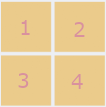
\includegraphics[width=.5\textwidth,height=.5\textheight,keepaspectratio]{images/numbering_board_2x2.PNG}
\end{figure}
\sethebrew

\begin{comm}
    \label{ comm: indexing board game}
    מספור  משורה ראשנה משמאל עד לסוף השורה ראשונה מימין ורק אז לרדת לשורה הבאה, היה
    שיטת המספור הקבוע בפרויקט זה עבור משחקים על לוח.
\end{comm}

לאחר מספור שכזה נוכל לומר שלחיצה על משבצת 
$1$
וקטור שינוי שלה נסמן ב
$t_1$
מתאר את עלו צמתים יכול שינוי.
$
    t_1 = 
    \begin{bmatrix}
        1 \\
        1 \\
        0 \\
        1 \\
    \end{bmatrix}
$

כדומה
עבור גרף באיור
\ref{fig:numbering_graph}
מתקבל וקטור שינוי של צומת 
$1$
כך
$
    t_1 = 
    \begin{bmatrix}
        1 \\
        0 \\
        1 \\
        1 \\
    \end{bmatrix}
$

\begin{figure}[ht]
    \caption{\R{גרף ממוספר}}
    \label{fig:numbering_graph}
    \unsethebrew
    \centering
    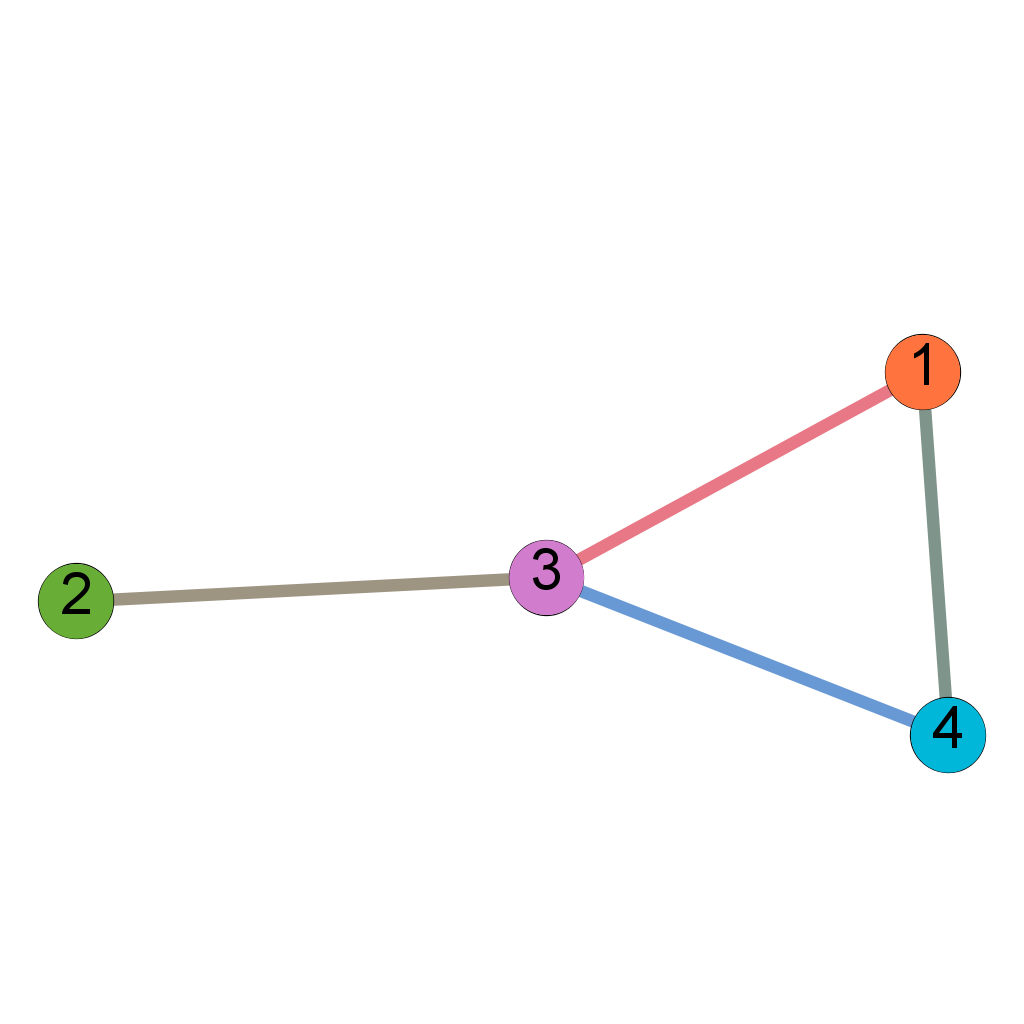
\includegraphics[width=.7\textwidth,height=.7\textheight,keepaspectratio]{images/numbering_graph.PNG}
\end{figure}
\sethebrew

\begin{definition}
    אפשר להגדיר את 
    וקטור השינוי
    של 
    לחצן
    $i$
    שנסמן ב
    $\vec{t_j}$
    וקטור
    שייך 
    לשדה 
    $\Zn$
    כאשר 
    $F_2$
    שדה בינארי
    ו 
    $n$
    הינו מספר הלחצנים.

    נגדיר שערכיו
    $t_{i,j} = 1$
    עבור
    לחצנים
    $j$
    שכנים עליו ועל עצמו
    ושאר ערכי וקטור שווים ל
    $0$.
\end{definition}

\begin{comm}
    היות ווקטור שינוי שדה
    $\Zn$
    חיבור בין וקטורים הינו חיבור בין האינדקסים מודול 
    $2$
    וכפל בסקלר
    הוא לכפול את כל ערכי וקטור בסקלר
    כאשר הסקלרים יכולים להיות
    $0$
    או 
    $1$
\end{comm}

בעזרת וקטורי השינוי אפשר לתאר תוצאה של קומבינציות של לחיצות
בעזרת צירוף לינארי של וקטורי שינויים.
את המצב המתקבל נוסיף למצב הקיים ונקבל את השינוי שנוצר בלחיצה של כפתורים.
נדגים רעיון זה על איור
\ref{fig:start graph presses}
.

נניח שצומת 1 היא יחידה שדלוקה.
\\
נרצה להראות איך הגרף יראה עם ילחצו על כפותרים 
$1, 3$.

\begin{figure}[ht]
    \caption{\R{מצב התחלתי}}
    \label{fig:start graph presses}
    \unsethebrew
    \centering
    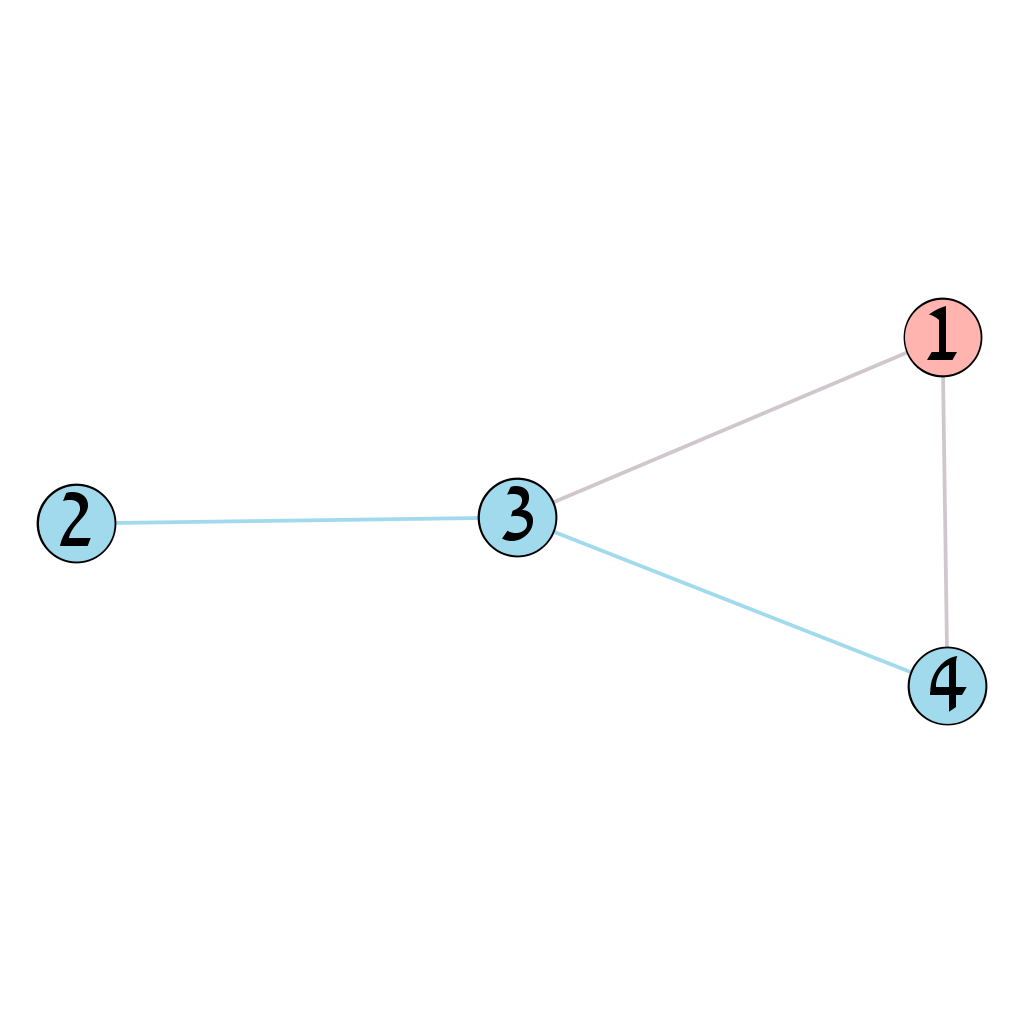
\includegraphics[width=.7\textwidth,height=.7\textheight,keepaspectratio]{images/graph_presses.png}
\end{figure}
\sethebrew

$
    t_1 + t_3 = 
    \begin{bmatrix}
        1 \\
        0 \\
        1 \\
        1 \\
    \end{bmatrix}
    +
    \begin{bmatrix}
        1 \\
        1 \\
        1 \\
        1 \\
    \end{bmatrix}
    =
    \begin{bmatrix}
        0 \\
        1 \\
        0 \\
        0 \\
    \end{bmatrix}
$

ומצב התחלתי שמתואר באיור נסמן ב
$S_0$
לכן מתקבל

$
    S_0 + t_1 + t_3 = 
    \begin{bmatrix}
        1 \\
        0 \\
        0 \\
        0 \\
    \end{bmatrix}
    +
    \begin{bmatrix}
        0 \\
        1 \\
        0 \\
        0 \\
    \end{bmatrix}
    =
    \begin{bmatrix}
        1 \\
        1 \\
        0 \\
        0 \\
    \end{bmatrix}
$

וקטור התוצאה שהתקבל אכן תואם לתוצאה המצופה
מתואר באיור 
\ref{fig:start graph presses solution}.

\begin{figure}[ht]
    \caption{\R{מצב לאחר ביצוע הלחיצות}}
    \label{fig:start graph presses solution}
    \unsethebrew
    \centering
    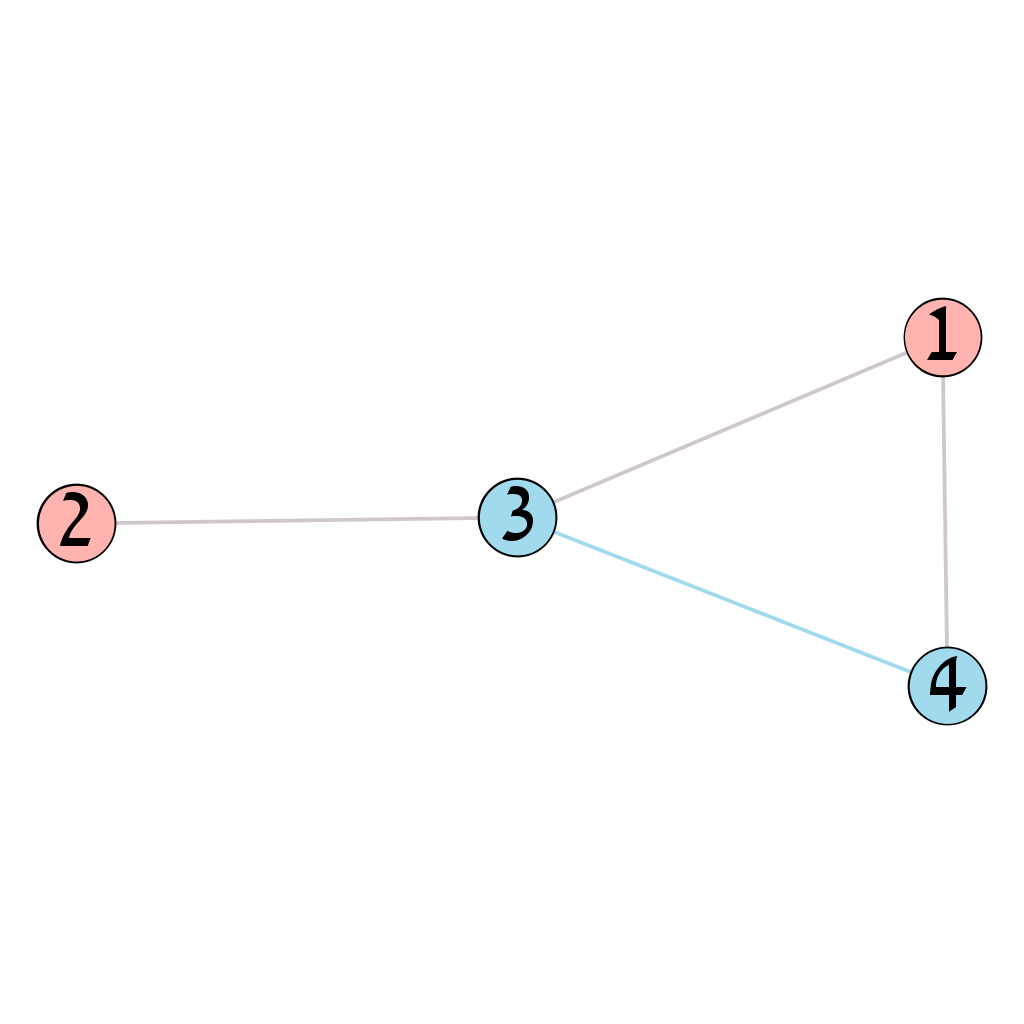
\includegraphics[width=.7\textwidth,height=.7\textheight,keepaspectratio]{images/graph_presses_solve.png}
\end{figure}
\sethebrew

\begin{lemma}
    \label{lemma: sum same change vect}
    מספר זוג של לחיצות אינו משנה את מצב הלוח
\end{lemma}
היות 
ואנחנו עובדים על שדה מודול 
$2$
$t_i + t_i = \vec{0}$

\begin{comm}
    \label{comm: press is uneven presses}
    לפי למה
    \ref{lemma:  sum same change vect}
    מספר הלחיצות על אותו לחצן אינו משנה 
    לחצן עכשיו 
    לחוץ אם נלחץ מספר אי זוגי של פעמים 
    כי מספר לחצות הזוגיות לא שינו את הלוח.

    לכן בהמשך שנציג את הפתרון נסמן לחצות על לחצן 
    $i$
    ב
    $x_i$
    אז 
    $x_i = 1$
    יסמן את המצב שלוחצים על הלחצן אבל לא ישנה כמה פעמים נלחץ הלחצן 
    כל עוד הוא נלחץ מספר אי זוגי של פעמים.
\end{comm}

נשים לב שעבור איך שהגדרנו את המשחק 
\L{Light out}
המשחק מתחיל כשכול
נורות דלוקות או כבויות
ומטרה היא לכבות או להדליק את כל נורות
כלומר לעבור ממצב דלוק לכבוי או ההפך.

אין באמת משמעות בין עם להתחיל את המשחק שכל הלחצנים דלוקים ולנסות לכבות אותם או ההפך ההבדל רק
מה המשמעות שנותנים לערכים
$0 ,1 $.

מפרק זה נגדיר שאנחנו פותרים את המשחק שלוח התחלתי כולו באפסים
ומטרה להגיע ללוח שכולו אחדים.

מתיאור שכזה מובן כי 
$S_0$
זהו וקטור אפסים לכן כדי לתאר את ממצב התחלתי
למצב לצירוף לינארי של וקטורי שינוי 
אין צורך לחבר בין מצב התחלתי וצירוף לינארי
היות ומצב התחלתי הוא כולו וקטורי אפס
מתקיים:

\begin{equation}
    \label{eq: sum change vectors}
    S_0 + \sumi{j} a_i \vec{t_j} =  \sumi{j} a_j \vec{t_j}
\end{equation}

בעקבות כך ניתן לתאר את בעיית המשחק לצורה הבאה:

\begin{equation}
    \label{eq: lin eq for solving problem}
    \sumi{j} a_j \vec{t_j} = \vec{1}
\end{equation}

כאשר
$\vec{1}$
וקטור שכל ערכיו אחדים
ו
$n$
מספר הצמתים בגרף.

תיאור שכזה מדגיש מספר תכונות 

\begin{lemma}
    סדר הלחיצות לא משנה את התוצאה הסופית
\end{lemma}
נשים לב שאם ידוע קבוצת לחיצות ממצב התחלתי הערך של משבצת מסוימת נקבע לפי 
הערך של וקטור תוצאה
בנוסחה
\ref{eq: sum change vectors}.
נשים לב שתוצאת הסכום איננה תלויה בסדר הלחיצות של הוקטור. 

מערכת משוואות 
שמתוארת בנוסחה
\ref{eq: lin eq for solving problem}
אפשר לתאר במספר צורות ונפוצה מבניהם היא
בעזרת מטריצה כמו שמתואר 
בנוסחה 
\ref{eq: matrix eq for solving problem}.

\begin{equation*}
    \begin{bmatrix}
        t_1 & t_2 & \cdots & t_n
    \end{bmatrix}
    \begin{bmatrix}
        a_1 \\
        a_2 \\
        \cdots \\
        a_n \\
    \end{bmatrix}
    =
    \begin{bmatrix}
        1 \\
        1 \\
        1 \\
        1 \\
    \end{bmatrix}
\end{equation*}
\begin{equation}
    \label{eq: matrix eq for solving problem}
    \begin{bmatrix}
        t_{1,1} & t_{1,2} & \cdots & t_{1,n} \\
        t_{2,1} & t_{2,2} & \cdots & t_{2,n} \\
        \cdots & \cdots & \cdots & \cdots\\
        t_{i,j} & t_{i,2} & \cdots & t_{i,n} \\
        \cdots & \cdots & \cdots & \cdots\\
        t_{n,1} & t_{n,2} & \cdots & t_{n,n} \\
    \end{bmatrix}
    \begin{bmatrix}
        x_1 \\
        x_2 \\
        \cdots \\
        x_n \\
    \end{bmatrix}
    = 
    \begin{bmatrix}
        1 \\
        1 \\
        \cdots \\
        1 \\
    \end{bmatrix}
\end{equation}

נשים לב שלמטריצה
$A$
במשוואה
\ref{eq: matrix eq for solving problem}
מתקבל ש
$A_{i,j} = 1$
כאשר 
$i, j$
צמתים שהם שכנים או זהים
$i = j$
לכן אפשר להגדיר את המטריצה כך.

\begin{definition}
    \label{def: neighbor matrix}
    מטריצה שמתארת את משחק תקראה מטריצת שכנויות של משחק.
\end{definition}


\begin{comm}
    \label{comm: symetic matrix}
    היות וכל צומת שכנה היא שכנה אחד לשני לכן במטריצה
    סימטרית
\end{comm}

המטריצה  המתקבלת מגרף באיור 
\ref{fig:start graph presses solution}:

\[
    \begin{bmatrix}
        1 & 0 & 1 & 1\\
        0 & 0 & 1 & 0\\
        1 & 1 & 1 & 1\\
        1 & 0 & 1 & 1\\
    \end{bmatrix}
\]


\begin{definition}
    \label{ def: solution vector}
    תהי משחק ומערכת משוואת שמתארת אותו מצורה 
    \ref{eq: matrix eq for solving problem} 
    נגדיר את וקטור פתרון כאוסף הלחצנים ומצב להגיע לפתרון
    ונסמן אותו ב
    $\vec{x}$
\end{definition}

הגדרה 
\ref{ def: solution vector}
מתכוונת שאם מתקבל
$\vec{x}$
וקטור פתרון של המערכת 
ו
$x_i = 1$
אז המשמעות שכדי לפתור את המשחק
צריך ללחוץ על לחצן 
$i$.
\\
בנוסף 
$\vec{x}$
אחד הפתרונות אתכן והיו כמה.

\begin{definition}
    \label{def: standard solution}
    שיטת פתרון בעזרת יצירת  מטריצה שכנויות על ידי וקטורי שינויים תקראה שיטה הסטנדרטית

    בגלל שאמרנו שנציג כמה שיטות ונרצה להתייחס לשיטה זה בשם לכן קראנו שיטה סטנדרטית
\end{definition}

תוצאה דומה אפשר לראות בפרק מהספר
\cite{B2}.
מרגע שהצלחנו לתאר את הבעיה מערכת משוואות לינארית
על שדה
$\Zn$
מכן נוכל להיעזר בכלים של אלגברה לינארית כדי למצוא את הפתרון כמו מציאת פתרון בעזרת דירוג,
מציאת מטריצה פסאדו הפוכה וכולי. 

\begin{comm}
    \label{comm: for board too many variables}
    עבור לוח 
$[n \times n]$
כמות הלחצנים 
$n^2$
ולכן גודל המטריצה שתוארה במשוואה
\ref{eq: matrix eq for solving problem}
היא 
$[n^2 \times n^2]$
\end{comm}

כלומר כמות הזיכרון שצריך כדי לשמור מטריצה ללוח ריבועי שאורך צלע הוא
$n$
דורש לשמור מטריצה עם 
$n^4$
ערכים
.

\subsection{פתרון בעזרת שיטה הספרדית}
הצגנו גישה פתרון
בגישה הסטנדרטית 
כפי שתיארנו
בהגדרה
\ref{def: standard solution}.
נרצה להראות שיטה נוספת למציאת פתרון.
הפתרון שנציג הינו חלק מחידה שניתנה למתמטי.
שיטת הפתרון שהוא מציג נובעת מהערה 
\ref{comm: for board too many variables}
שכמות המידע שצריך לשמור גדל בקצב 
$n^4$
כאשר
משחק הוא על לוח ריבועי ש
$n$
מייצג
כמות הלחצנים לשורה.
הצורך לצמצום כמות המשתנים נבעה מצורך פרקטי כי לא היה מספיק זיכרון לאכלס את כל מידע 
באותה תקופה ולכן שיטה זה הומצאה.

במאמר 
\cite{B1}
מציג שיטה שמציאה פתרון עם מערכת משוואות לינארית אחרת שמובילה גם היא לפתרון.
מערכת משוואת לינארית שמאמר 
\cite{B1}
מתאר ממדי
$n \times n $.
כלומר כמות הערכים המטריצה המתקבלת שווה
ל
$n^2$
שקטנה משמעותית 
ממערכת המתקבלת בשיטה הסטנדרטית.

בפרק זה נציג את הגישה שמתוארת 
\cite{B1}
נתאר כמה הבחנות שיסתמכו ששני הגישות שקולות ושגישה החדשה הינה רק אופטימיזציה
ספציפית לצורה של מטריצה הנתונה.
את הגישה החדשה ניקרא לאורך כל הפרק הגישה הספרדית.

\begin{definition}
    \label{def: spanish way}
    גישה הספרדית גישה פתרון שניה שנציג בעבודה זה.
\end{definition}

נתאר את הגישה הספרדית 
זה הינה גישה שמתאימה לכל גודל של לוח משחק.
כדי להקל על תיאור 
בעזרת דוגמה על לוח 
$3 \times 3$

נניח שאיור 
\ref{fig: 3 x 3 board indexed}
מתאר את הלוח הנתון כאשר המשבצות הינן הלחצנים ומספור זה אינדקסים הערה 
\ref{ comm: indexing board game}
רק שהפעם נתחיל את המספור מ
$0$

\begin{figure}[ht]
    \caption{לוח 
    $3 \times 3$
    עם אינדקסים}
    \label{fig: 3 x 3 board indexed}
    \unsethebrew
    \centering
    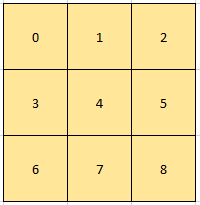
\includegraphics[width=.3\textwidth,height=.3\textheight,keepaspectratio]{images/3x3_board_index.PNG}
\end{figure}
\sethebrew

שיטת הפתרון של מאמר הספרדי הינה להתחל את הלוח עם משתנים ולמלאות את הלוח במשתנים עלו.
לאחר שכל הלוח מלא מתקבלים 
$n$
משוואות במקרה של דוגמה 
באיור 
\ref{fig: 3 x 3 board indexed}
כמות המשוואות תהיה
$3$
וכל משוואה תהיה עם 
$n$
נעלמים
ולכן נקבל מערכת משוואת שמטריצה המייצגת הינה מסדר 
$n \times n$

שיטת הספרדית מתחיל בכך
שממלאים את השורה העליונה במשתנים
כפי שמתואר באיור 
\ref{fig: 3 x 3 board init spanish}.
לאחר מכן עוברים שורה שורה 
וממלאים אותה במשתנים שמשפיעים על הלחצן.

בשלב זה נסביר את אופן המילוי ומשמעות המשתנים.
נסמן ב
$x_i = 1$
אם נילחץ על לחצן 
$i$.
נזכיר לפי הערה 
\ref{comm: press is uneven presses}
שלחצן נחשב ללחוץ עם הוא נלחץ מספר אי זוגי של פעמים 
כי מספר זוגי מחזיר את הלוח למצב המקורי לכן
אנחנו מתייחסים רק האם נלחץ הלחצן או לא.

אם נתייחס לכל הלחצנים כווקטור מסודר לפי אינדקס
$i$
נקבל 
$\vec{x}$
כפי שהגדרנו בהגדרה 
\ref{ def: solution vector}.

היות ומטרה לשנות את מצב הלחצנים
למצב 
$1$
כלומר צריך שכמות לחיצות על לחצנים שמשפיעים על 
משבצת סכום במודול
$2$
היה 
$1$.

נדגים
על כמה לחצנים מאיור  
\ref{fig: 3 x 3 board indexed}.
מצב הלחצן תלוי האם הלחצנים 
סמוכים לו  ועצמו לחוצים .
\\
עבור 
לחצן 
$0$.
מתקבלת המשוואה:

\[ x_0 + x_1 + x_3 = 1\]

ועבור לחצן 
$3$:

\begin{equation}
    \label{eq: cond eq}
    x_0 + x_3 + x_4 + x_6 = 1
\end{equation}


וכך ניתן להגדיר אילוצים לכל הלחצנים.

\begin{definition}
    \label{ def: depndeciy equation}
    המשוואה המתקבלת
    עבור לחצן 
    $i$
    מחיבור מודל 
    $2$
    עם נלחצו לחצנים המשפעים על לחצן 
    תקראה
    משוואת אילוצים על לחצן 
    $i$
    
    משוואה 
    \ref{eq: cond eq}
    הינה משוואת האילוצים שללחצן
    $3$.
\end{definition}

עבור משחק לוח
ריבועי באורך שורה 
$n$
שהלחצנים ממספרים לפי הערה
\ref{ comm: indexing board game}
ניתן לנסח בנוסחה פשוטה:
\begin{equation}
    \label{eq: depndeciy equation}
    x^*_{i - n} + x^*_{i - 1} + x^*_{i} + x^*_{i + 1} + x^*_{i + n} = 1
    \hspace{10pt}
    x^*_i =
    \begin{cases}
        x_i & \text{if $i \in [1,n^2]$} \\
        0 & \text{otherwise}
    \end{cases}
\end{equation}

\begin{figure}[ht]
    \caption{לוח 
    $3 \times 3$
    מאותחל}
    \label{fig: 3 x 3 board init spanish}
    \unsethebrew
    \centering
    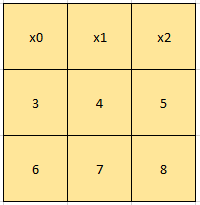
\includegraphics[width=.3\textwidth,height=.3\textheight,keepaspectratio]{images/3x3_first_row.PNG}
\end{figure}
\sethebrew

לאחר שהגדרנו את משוואת האילוצים נסביר כיצד למלאה 
את השורות הנותרות לפי השיטה הספרדית.
\\
כל לחצן ימלא לפי משוואת האילוצים של הלחצן שמעליו.
\\
כלומר 
כדי למלאה את לחצן 
$3$
נסתכל על משוואת האילוצים של לחצן 
$0$.

\[ x_0 + x_1 + x_3 = 1\]

ניזכר כי המשוואה שהתקבלה הינה על שדה מודול
$2$.
לכן בעזרת העברת אגפים מתקבל.

\[ x_3 = 1 + x_0 + x_1 \]

ונכתוב ערך זה בלחצן 
$3$
כמו שמתואר באיור 
\ref{fig: 3 x 3 board fill button 3}

\begin{figure}[ht]
    \caption{לוח 
    $3 \times 3$
    מילוי משבצת
    $3$}
    \label{fig: 3 x 3 board fill button 3}
    \unsethebrew
    \centering
    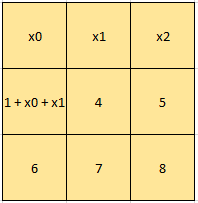
\includegraphics[width=.3\textwidth,height=.3\textheight,keepaspectratio]{images/3x3_fill_button_3.PNG}
\end{figure}
\sethebrew

נשים לב שבעזרת גישה שתיארנו כרגע נוכל למלאה כל השורה שניה.
כל שורה תלויה בשורה מלפניך לכן כך נוכל למלאה את כל השורות 
כמו שמתואר באיור 
\ref{fig: 3 x 3 board fill intire board}

נדגים מילוי משבצת
$6$
משורה שלישית לכן נצטרך ששורה
שניה חושבה.
\\
נסתכל על משבצת מעל 
כלומר משבצת 
$3$
ונסתכל למה שווה משוואת האילוצים שלה:

\[ x_0 + x_3 + x_4 + x_6 = 1 \]

לכן 

\[ x_6 = 1 + x_0 + x_3 + x_4  \]

היות ושורה שניה מולאה וידוע שערך משבצות 
באותה שורה: 

\begin{align*}
    x_3 &= 1 + x_0 + x_1 \\
    x_4 &= 1 + x_0 + x_1 + x_2
\end{align*}
    


נציב ערכים אילו

\begin{align*}
    x_6 &= 1 + x_0 + (1 + x_0 + x_1) + (1 + x_0 + x_1 + x_2) \\
    x_6 &= 1 + x_0 + x_2
\end{align*}

\begin{figure}[ht]
    \caption{לוח 
    $3 \times 3$
    מלאה}
    \label{fig: 3 x 3 board fill intire board}
    \unsethebrew
    \centering
    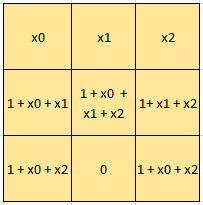
\includegraphics[width=.3\textwidth,height=.3\textheight,keepaspectratio]{images/3x3_fill_all.PNG}
\end{figure}
\sethebrew

כדומה נעשה לשאר הערכים.
התוצאה מתקבלת מתוארת באיור 
\ref{fig: 3 x 3 board fill intire board}

נבחין שלאחר שמילאנו את כל הלוח כמו שמתואר באיור 
\ref{fig: 3 x 3 board fill intire board}
נותרו לנו עוד 
$n$
משוואות אילוץ שתלויות בשורה אחרונה ולכן מאמר 
\cite{B1}
מציאה להוסיף שורה וירטואלית כדי להשתמש 
במשוואות עלו
כמו שמתואר באיור 
\ref{fig: 3 x 3 board fill with virtual}

\begin{figure}[ht]
    \caption{לוח 
    $3 \times 3$
    מלאה
    כולל שורה וירטואלית
    }
    \label{fig: 3 x 3 board fill with virtual}
    \unsethebrew
    \centering
    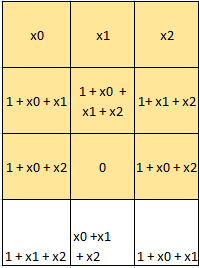
\includegraphics[width=.3\textwidth,height=.3\textheight,keepaspectratio]{images/3x3_fill_virtual.PNG}
\end{figure}
\sethebrew

המאמר טוען שהיות שורה זה לא באמת קיימת לכן
ערכי 
של משבצת המתקבלות 
חייב להיות שווה 
ל
$0$

ולכן קיבלנו 
$n$
משוואת על 
$n$
נעלמים 
כאשר בדוגמה שלנו 
$n=3$
לכן אפשר לנסות לפתור את המערכת הנתונה.

שיטה שתיארנו ביצע מעבר על שורות אפשר היה לעשות בניה דומה גם לעמודות.

המאמר 
\cite{B1}
מתאר מספר רב של פתרונות  בלוחות ריבועים בגדלים שונה ואפילו על לוחות מלבניים.
האתגר המרכזי בשיטה הספרדית היא להצדיק אותה למה יש שורה וירטואלית
והאם יש קשר בין שני השיטות.
בשלב זה נתרכז להראות את הקשר בין שיטה הספרדית ושיטה שהצגנו בפרק הקודם.

\begin{theorem}
    מטריצה המיצג של מערכת המשוואות האילוצים היא מטריצת שכנויות
    \ref{eq: matrix eq for solving problem}.
\end{theorem}
משוואות האילוצים פורמלית היא לב השיטה הספרדית
מכיוון שהתקדמות בשורות מבוססת על המשוואות עלו.

אם נפרוס את משוואת האילוצים נקבל גם מערכת משוואת שפותרת את המשחק
אבל כמות המשואות הינה 
$n^2$.
נבחין שאם נציג אותם כמטריצה כאשר כל משוואת אילוצים מסודר לפי סדר הלחצנים נקבל את מטריצה שכנויות שהצגנו במשוואה 
\ref{eq: matrix eq for solving problem}
מתקבל ממשוואת האילוצים שמשתנה 
$x_i$
מופיעה בהם
באותם אינדקסים 
$j$
בווקטור שינוי
של לחצן 
$i$
כך שבערך 
$t_{i,j}$
מתקבל ערכים 
שווים
ל
$1$
ולכן מתקבלת אותה מטריצה.

נדגים זאת על לוח 
$2 \times 2$
שמתואר באיור 

\begin{figure}[ht]
    \caption{לוח 
    $3 \times 3$
    מלאה
    כולל שורה וירטואלית
    }
    \label{fig: 2 x 2 board}
    \unsethebrew
    \centering
    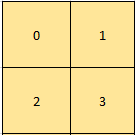
\includegraphics[width=.3\textwidth,height=.3\textheight,keepaspectratio]{images/2x2_board.PNG}
\end{figure}
\sethebrew

וקטורי השינויים:

\[
   t_0 = 
    \begin{bmatrix}
        1 \\
        1 \\
        1 \\
        0 \\
    \end{bmatrix},
    t_1 = 
    \begin{bmatrix}
        1 \\
        1 \\
        0 \\
        1 \\
    \end{bmatrix},
    t_2 = 
    \begin{bmatrix}
        1 \\
        0 \\
        1 \\
        1 \\
    \end{bmatrix},
    t_3 = 
    \begin{bmatrix}
        0 \\
        1 \\
        1 \\
        1 \\
    \end{bmatrix},
\]
לכן
המטריצה מהצורה:
\[
    \begin{bmatrix}
        1 & 1 & 1 &0 \\
        1 & 1 & 0 & 1 \\
        1 & 0 & 1 & 1 \\
        0 & 1 & 1 & 1 \\
    \end{bmatrix},
\]

ומשוואת האילוצים
מהצורה 

\begin{align*}
    x_0 + x_1 + x_2 &= 1\\
    x_0 + x_1 + x_3 &= 1\\
    x_0 + x_2 + x_3 &= 1\\
    x_1 + x_2 + x_3 &= 1
\end{align*}

תעלומה נוספת בשיטה הספרדית היא למה צריך שורה וירטואלי, למה ערכה 
שווה ל
$0$
ואיך המערכת משוואת שלו מצטמצמת ל
$n$
משתנים
\\
הסבר לתופעה זה
ניתן בעזרת הצגה המטריצה
נראה זאת על מטריצה 
של משחק 
על לוח 
$3 \times 3$

נשים לב ששיטה הספרדית מדרג את המטריצה מורחבת 
$[M | \vec{1}]$.

\begin{center}
    \begin{tabular}{|ccccccccc|c|}
        \hline
        1& 1& 0& 1& 0& 0& 0& 0& 0& 1 \\
        1& 1& 1& 0& 1& 0& 0& 0& 0& 1 \\
        0& 1& 1& 0& 0& 1& 0& 0& 0& 1 \\
        1& 0& 0& 1& 1& 0& 1& 0& 0& 1 \\
        0& 1& 0& 1& 1& 1& 0& 1& 0& 1 \\
        0& 0& 1& 0& 1& 1& 0& 0& 1& 1 \\
        0& 0& 0& 1& 0& 0& 1& 1& 0& 1 \\
        0& 0& 0& 0& 1& 0& 1& 1& 1& 1 \\
        0& 0& 0& 0& 0& 1& 0& 1& 1& 1 \\
        \hline
    \end{tabular}
\end{center}

נבחין כי מילוי משבצת 
$j$
בשיטה הספרדית מחייבת פעולת הצבה של משבצת
$k$
שכבר מולאה פעולה זה שקולה 
לחיבור עם אות שורה במטריצה, כלומר אפשר לתאר זאת על ידי פעולת שורה 
המתוארת כך,
\[ j \leftarrow j + k \]

תקבל ששיטה הספרדית הינה 
שיטה חכמה לדרג את הבעיה
עד שנותר 
$n$
משוואות.
נבחין שמשבצת שחושבו
שהם משבצות 
מ
$3$
עד 
$8$
באיור
\ref{fig: 3 x 3 board indexed}
בשיטה הספרדית
שקולה לשורה 
$i-3$
במטריצה המורחבת המדורגת
באיור
\ref{fig: matrix after spanish}

\begin{figure}
    \caption{המטריצה לאחר דירוג לפי שיטה הספרדית המתקבלת
        מלוח 
        $3 \times 3$}
    \label{fig: matrix after spanish}
    \begin{center}
        \begin{tabular}{|ccccccccc|c|}
            \hline
    1& 1& 0& 1& 0& 0& 0& 0& 0& 1 \\
    1& 1& 1& 0& 1& 0& 0& 0& 0& 1 \\
    0& 1& 1& 0& 0& 1& 0& 0& 0& 1 \\
    1& 0& 1& 0& 0& 0& 1& 0& 0& 1\\
    0& 0& 0& 0& 0& 0& 0& 1& 0& 0\\
    1& 0& 1& 0& 0& 0& 0& 0& 1& 1\\
    0& 1& 1& 0& 0& 0& 0& 0& 0& 1\\
    1& 1& 1& 0& 0& 0& 0& 0& 0& 0\\
    1& 1& 0& 0& 0& 0& 0& 0& 0& 1\\
            \hline
        \end{tabular}
    \end{center}
\end{figure}

לסיכום השיטה הספרדית היא שקולה לדירוג חכם של המטריצה.
אפשר לומר שמספיק היה לפתור רק 
$n$
המשואות של שיטה הספרדית כדי למצוא את הפתרון של המשחק.

לפי חישוב סיבוכיות
לדרג מטריצה 
כללית
בגודל 
$n^2 \times n^2$
זה 
$O(n^2 \cdot n^4) = O(n^6)$.

דירוג בעזרת שיטה הספרדית אומרת
שעל כל עמודה 
וקטור עמודה 
של מטריצת שכנויות
יש לכל יותר
$5$
ערכים ששווים 
$1$.
כל החוכמה בדירוג בשיטה הספרדית היא 
שפעולות השורות הם על משתנים שכבר דורגו
לכן 
כמות הפעולות שורות לא משתנה.
לכן דירוג שורה היה חיבור 
של עד כ
$5$
שורות
לכן הסיבוכיות 
$O(n^2 \cdot n^2) = O(n^4)$
.

לדרג את
$n$
משתנים  
הנותרים
הוא בסיבוכיות 
$O(n \cdot n^2) = O (n^3)$.

ננסה להראות זאת בפועל על ידי חישוב זמני חישוב.

\begin{figure}[ht]
    \caption{ 
    גרף מתאר ביצועים על לוח ריבועי גודל שורה מול זמן
    }
    \label{fig:prefofmance_diagram}
    \unsethebrew
    \centering
    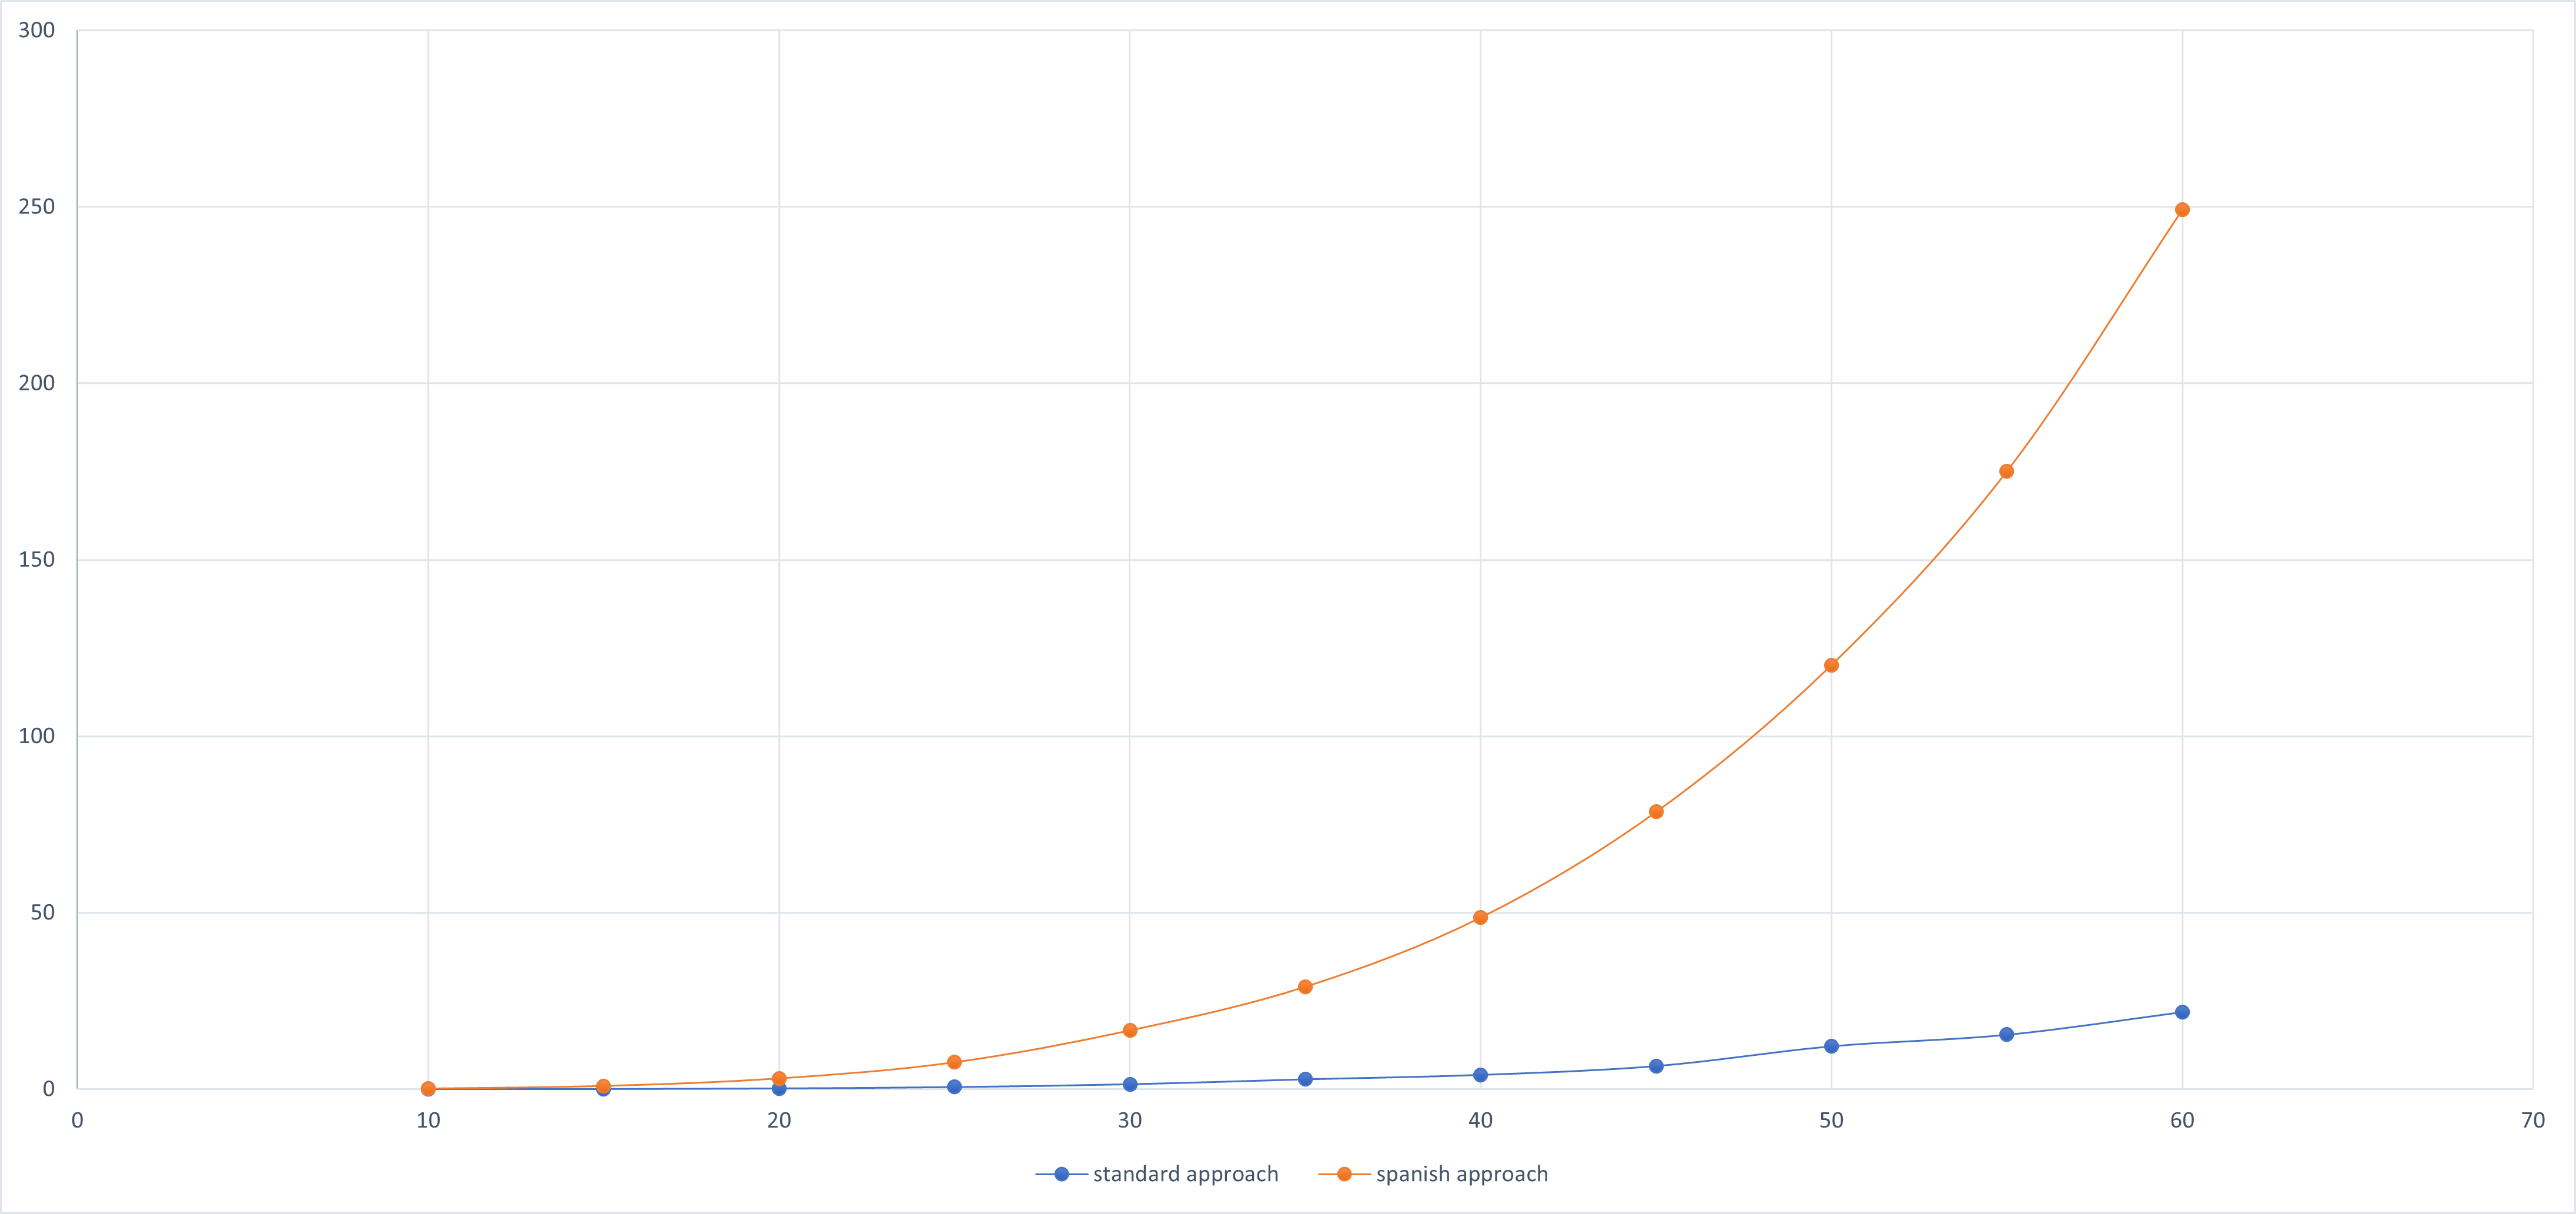
\includegraphics[width=\textwidth,height=\textheight,keepaspectratio]{images/benchmark.png}
\end{figure}
\sethebrew

באיור 
\ref{fig:prefofmance_diagram}
אפשר לראות ביצועים
של שני האלגוריתמים ציר 
ה
$x$
גודל שורה של לוח המלבני
הרצנו על 
לוח בגדלים 
מ
$10$
עד 
$60$
משבצות.
ציר ה
$y$
זמן שלקח 
בשניות
\\
לפי התוצאות של איור 
\ref{fig:prefofmance_diagram}
ניראה 
שגישה הספרדית שבתאוריה יותר אופטימליות לוקחת יותר זמן.
אחת הסיבות לקח 
שפונקציה שפותרת מערכת משוואות הינה פונקציה של ספירה שנעזרתי וכנראה יש מימוש אופטימלי לפתרון הבעיה שאפילו 
ששיטה הספרדית מקטינה את כמות 
המשתנים היא אינה יכולה להתחרות במימוש אופטימלי שממשה בספריה.

\newpage
\section{הוכחת  קיום פתרון עבור כל גרף}
עד כה הסתכלנו על שני גישות שונות למציאת פתרון
אבל שאלה טבעית לשאול היא האם בכלל קיים פתרון למשחק על לוח כלשהו?
אחת הדרכים לענות על שאלה שכזה היא פשוט לקחת את הלוח ולפתור בעזרת 
דרכי הפתרון שהצגנו.
אחת הבעיות בגישה של לחפש פתרון על לוח כלשהו היא 
נניח ואנחנו רוצים לממש את המשחק האורות שמיצר לוחות אקראיים, היות ולא בהכרח ידוע אם קיים פתרון 
נצטרך לבדא שקיים פתרון על כל לוח בעזרת אלגוריתמים למציאת פתרון שלוקח זמן 
אתכן והלוח ללא פתרון נצטרך לחפש לוח אקראי אחר
מה שיגרום לתהליך יצירת משחק להיות איטי.
לכן, נרצה בשיטה מתמטית להוכיח לעבור איזה משחקים יש פתרון.
בנוסף שאלה נוספת שאפשר לשאול היא כמה פתרונות יש ללוח.
מספר הפתרונות של הלוח יכול להעיד האם הלוח יותר קל או קשה לשחקן שמנסה לפתור אותו
לבד ללא אלגוריתם.
בפרק זה נענה על השאלות הללו.

אחד המקומות ששאלה זה נשאלה היא בספר 
\cite{B3},
בעבודתנו נראה הוכחה קצת שונה בעזרת הכלים שפיתחנו.

\begin{definition}
    \label{def:inner_mul}
    נגדיר פעולה 
    בין שני וקטורים ב
    $\Zn$
    ניקרא לה מכפלה סקלארית
    תסומן 
    $x \cdot y$
    ונגדיר אותה כך:
    \\
    תהי 
    $\vec{x}, \vec{y} \in \Zn$
    אז 
    \[
        \vec{x} \cdot \vec{y} = 
        \begin{bmatrix}
            x_1 \\
            x_2 \\
            \cdots \\
            x_n \\
        \end{bmatrix}
        \cdot 
        \begin{bmatrix}
            y_1 \\
            y_2 \\
            \cdots \\
            y_n \\
        \end{bmatrix}
        = 
        x_1 y_1 + x_2 y_2 + \cdots x_n y_n
    \]
    כאשר 
    פעולת חיבור בין האיברים 
    הינה 
    חיבור מודול
    $2$
\end{definition}

\begin{comm}
    \label{comm:not_really_inner_mul}
    המכפלה הסקלארית שהגדרנו ב
    \ref{def:inner_mul}
    אינה מכפלה פנימית היות ותכונה 
    $<\vec{u},\vec{u}> = 0 \Leftrightarrow \vec{u} = \vec{0} $
    לא מתקיימת.
\end{comm}

דוגמה 
שמסבירה את הערה
\ref{comm:not_really_inner_mul}:

\[
    \begin{bmatrix}
    1 \\
    1 \\
    \end{bmatrix}    
    \cdot 
    \begin{bmatrix}
    1 \\
    1 \\
    \end{bmatrix} 
    = 1 + 1 = 0
\]

\begin{comm}
    וקטורים 
    $\vec{x}. \vec{y} \in \Zn $
    יקראו מאונכים אחד לשני נסמן זאת 
    $\vec{x} \perp  \vec{y}$
    אם המכפלה הסקלארית שהלם שווה 
    ל
    $0$
    $\vec{x} \cdot \vec{y} = 0$
\end{comm}

\begin{theorem}
    \label{the: Nul A and Col AT}
    תהי מטריצה 
    $A \in {Z_2}^{m \times n }$
    אז 
    $ColA^T \perp Nul A$
    $ColA \perp Nul A^T$
\end{theorem}

ידוע שתכונה זה מתקיימת 
ב
מטריצה 
$A \in R^{m \times n}$
ההוכחה 
ל
$ {Z_2}^{m \times n}$
זה
פרט ל
למכפלה הפנימית 
שדורשת 
לבצע על תוצר 
ב
$R^{m \times n}$
עוד 
מודל 
$2$.
היות ותוצר של מכפלה פנימית הינו אפס גם לאחר מודל 
$2$
היה 
$0$.

\begin{theorem}
    \label{thrm: clean game has solution}
    לכל משחק על גרף כאשר המצב התחלתי בו כל הנורות במצב 
    $0$
    קיים פתרון למשחק.
\end{theorem}
לפי 
שיטת פתרון סטנדרטית 
שהגדרנו
\ref{def: standard solution}
ניתן לתאר את פתרון המשחק על גרף בעזרת מטריצה
שכנויות לפי הגדרה 
\ref{def: neighbor matrix}.
מטריצה שכנויות
נסמן אותה ב
$A \in {Z_2}^{n \times n}$.

נזכיר כמה תכונות חשובות
\begin{enumerate}
    \item 
    מטריצה סימטרית לפי
    \ref{comm: symetic matrix}
    \item 
    $A$
    המטריצה הינה ריבועית.
    \item 
    האיברים על האלכסון
    מטריצה 
    $A$
    ערכם שווה ל
    $1$.
\end{enumerate}

כדי להראות שלמשחק יש פתרון 
צריך להראות שקיי פתרון למערכת
\[A \vec{x} = \vec{1} \]

במקרה ש 
$A$
מטריצה הפיכה אז קיים פתרון יחיד.
עבור המקרה שמטריצה אינה הפיכה 
כלומר 
$Nul A \neq \{ \vec{0}\}$
ניקח 
$\vec{x} \in Nul A$
כלומר 
$A\vec{x} = \vec{0} \\$
$\vec{x}^T A \vec{x} = \vec{x}^T\vec{0} = 0 \\$
נסמן 
$\vec{x} = [x_1, x_2, \cdots, x_n]^T$

\begin{multline}
    \label{eq: quadratic form}
        \vec{x}^T A \vec{x} = a_{1,1}x_1^2 + 2(a_{1,2} + a_{2,1})x_1x_2 + \cdots 2(a_{1,n} + a_{n,1})x_1x_n + \\
        + a_{2,2}x_2^2 +  2(a_{2,3} + a_{3,2})x_2x_3 + \cdots  + 2(a_{2,n} + a_{n,2})x_2x_n + \cdots
\end{multline}

היות ומטריצה סימטריות
$a_{i,j} = a_{j,i}$
לכן
מתקבל
\[a_{i,j} - a_{j,i} = a_{i,j} + \cdots + a_{j,i} = 1 \]
נזכיר כי תוצאות של פעולת חיבור וחיסור מודל 
$2$
זהות.

לכן
את המשוואה 
\ref{eq: quadratic form}
אפשר לפשט ל
\[ \vec{x}^T A \vec{x} = a_{1,1}x_1^2 + a_{2,2} x_2^2 +  a_{n,n} x_n^2\]

הבחנה נוספת לערך 
$0$
או
$1$
$x^2 = x$
לכן פישוט נוסף למשוואה 
\ref{eq: quadratic form}
אפשרי:
\[ \vec{x}^T A \vec{x} = a_{1,1}x_1 + a_{2,2} x_2 +  a_{n,n} x_n\]

לכן קיבלנו 
$ \vec{x}^T A \vec{x} = 0$
שמתקיים:
\[a_{1,1}x_1 + a_{2,2} x_2 +  a_{n,n} x_n = 0\]

כלומר 
$\vec{1} \perp  \vec{x}$
כאשר 
$x \in Nul A$
לפי משפט 
\ref{the: Nul A and Col AT}
מתקבל 
$\vec{1} \in Col A^T$
היות ומטריצה סימטרית 
$A^T = A$
לכן
$\vec{1} \in Col A$
והוכחנו שלמערכת
$A\vec{x} = \vec{1}$
יש פתרון.

\subsection{מספר הפתרונות עבור כל גרף}
הוכחנו שלכל משחק על גרף שמתחל עם כל לחצנים במצב 
$0$
יש פתרון ניזכר שסדר לחיצות
אינו משנה את התוצאה על הלוח לכן אם נילחץ על הלחצנים בסדר כלשהו 
לפי פתרון נקבל גרף כולו דלוק.

השאלה  שנשאל בפרק זה מה אפשר לומר על מספר פתרונות מפיתוח שעשינו.
נציין קודם שניקרא לשני פתרונות שונים אם קיים לפחות לחצן אחד שמבדיל בין הפתרונות 
כלומר קיים לחצן ששייך לפתרון ראשון ולא שייך לפתרון שני כפי שציינו קודם סדר
לחיצות לא משנה את הפתרון.
לכן פתרון הינו קבוצה של לחצנים.
בנוסף נזכר לפי הערה
\ref{comm: press is uneven presses}
מספר אי זוגי של לחיצות נחשב ללחיצה לכן מספר הלחיצות על אותו לחצן לא משנה 
אלה רק זוגיות של מספר לחיצות 
לכן לכל לחצן יש רק שני מצבים שיכול להיות 
לחוץ 
או לא.
כרגע נראה שקיים כמה פתרונות לדוגמא 
איור
\ref{fig: clic 3 node graph game}
המתאר משחק על גרף בו הצמתים כבויים.
היות וגרף הינו קליקה לכן לחיצה בודדת על אחד הצמתים תדליק את כל הלחצנים.

קבלנו 
$G = \{\{v_1\}, \{v_2\}, \{v_3\} \}$
היא קבוצת של פתרונות.
כלומר כבר הראינו שיש מקרים בהם יש יותר מפתרון אחד.

\begin{figure}[ht]
    \caption{משחק על גרף}
    \label{fig: clic 3 node graph game} 
    \unsethebrew
    \centering
    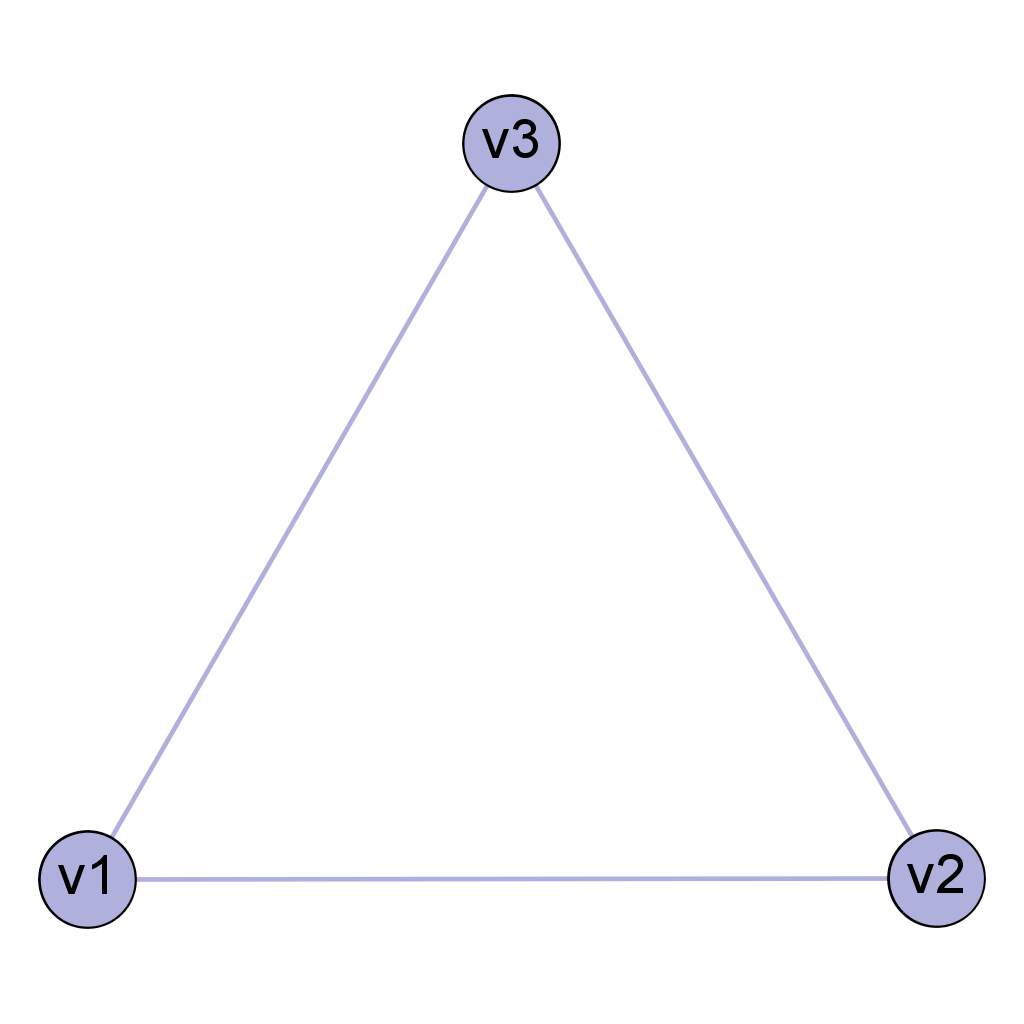
\includegraphics[width=.5\textwidth,height=.5\textheight,keepaspectratio]{images/clic_graph_3_node.png}
\end{figure}
\sethebrew

שאלה טביעת שנובעת כשגילנו שיש היא כמה פתרונות יש למשחק מסוים.

\begin{theorem}
    מספר הפתרונות של משחק 
    שווה ל 
    $2^{k}$
    כאשר 
    $k$
    שווה לדרגת החופש של מטריצה
    $A$
    של פתרון הסטנדרטי
\end{theorem}

היות לכל משחק ניתן להגיר מטריצת שכנויות של משחק שהגדרנו 
ב
\ref{def: neighbor matrix}
ופתרונות של משחק וקטורים
$X$
של מערכת
$A X = \vec{1}$
כאשר 
$A$
מטריצת שכנויות.
ידוע שקיים פתרון למשחק ואם הוא משחק שמתחיל שמצב כל הנורות הוא
$0$
אז יש משפט 
\ref{thrm: clean game has solution}.
שמוכיח שקיים פתרון.

היות ומניחים שיש כמה פתרונות אפשר לתאר את כל פתרונות כ
$x = x_n + x_0$
כאשר 
$x_n \in Nul(A)$ ,
$x_0$ 
פתרון פרטי שידוע שקיים 
ו
$x$
כל פתרונות הכללים.

לכן מספר פתרונות כללים שווה למספר פתרונות במרחב האפס.
ידוע שמספר פתרונות במרחב האפס תלוי לדרגת החופש ולכן מספר הווקטורים שפורשים
את מרחב האפס שווה לדרגת החופש שנסמן ב
$k$.
כמות הווקטורים במרחב זה שווה לכל וקטורים שניתן ליצור בצירוף לינארי 
$x = a_1 x_1 + a_1 x_1 + a_2 x_2 + \cdots + a_k x_k$
כאשר הערכים של
$a_i \in Z_2$
לכן 
לכל מקדם יכול להיות
$2$
ערכים
לכן כל הקונבנציות האפשריות 
$2^k$
ששווה
לכמות הווקטורים 
במרחב האפס וכמות הפתרונות השונים של המשחק.

הבחנה נוספת ומעניינת שנרצה לציין היא בנושא חסם עליון לכמות הפתרונות.
חסם עליון טריוויאלי לכמות המקסימלית של פתרונות היא 
$2^n$
פתרונות כאשר
$n$
שווה למספר הלחצנים כלומר לא יכול להיות יותר פתרונות מאשר כמות הלחיצות השונות האפשריות במשחק.

\begin{comm}
    עבור משחק לוח מלבני
    בגודל 
    $m \times n$
    קיים לכל יותר 
    $2^k$
    כאשר 
    $k = \min{m,n}$
    פתרונות שונים
\end{comm}
הערה זה נכונה לפי גישה פתרון הספרדית
שהגדרנו
\ref{def: spanish way}
ניתן לתרגם את משחק ל
$k$
משוואות 
ש
$k$
יכול להיות מספר שורות או עמודות 
לכן ניקח את המספר הקטן יותר.


\section{פתרון מינימלי עבור לוחות מלבניים}
בפרק זה נציג פתרון לסוג מסוים של פתרונות שרצינו להציע. סוג זה של פתרונות 
מביאים רמז וניראה שמקלים את משחק. הקלה שכזאת על משחק אולי 
יכולה ליצור ביטחון לשחקנים חדשים וכמובן לאפיין תכונות לסוג של פתרון של כזה.

\begin{definition}
משחקים על לוח שקיים פתרון שלחצנים 
שינו את מצב רק פעם אחת.
למשחקים כאלו נקראה משחק מנמליים.
\end{definition}

באיור 
\ref{fig: min sol 2x3}
ניתן דוגמא לפתרון מינמלי 
בלוח 
$2 \times 3$.
כשלוחצים על לחצנים 
$2, 3$
על לוח כל נורות נדלקות ואף 
אחת מהם לא נכבה באף שלב של לחיצה.

\begin{figure}[ht]
    \caption{פתרון מינמלי של משחק}
    \label{fig: min sol 2x3}
    \unsethebrew
    \centering
    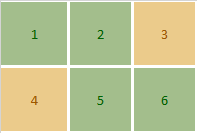
\includegraphics[width=.7\textwidth,height=.7\textheight,keepaspectratio]{images/min_sol_2x3.PNG}
\end{figure}
\sethebrew

השאלה שנפתור בפרק זה לאיזה לוחות קיים פתרון מינמלי כאשר מצב התחלתי הוא שכל הנורות במצב
$0$.

\begin{definition}
    \label{def: dead zone}
    אזור מת זהו אוסף לחצנים בלוח
    שלחיצה עליהם 
    גורמת לחצן שכבר השתנה בעבר להשתנות שוב
\end{definition}

איזורים מתים על איור 
\ref{fig: min sol 2x3}
נראה שלאחר לחיצה על
לחצן
$2$
האזור מת שנוצר מלחיצה הינו
$\{0,1,2,4,5\}$

\begin{comm}
    אזור מת שנוצר מלחיצה 
    הוא כל הלחצנים במרחק לכל יותר 
    $2$
    משבצות מלחצן שנלחץ
    כאשר המרחק הוא מרחק מנהטן כלומר כל צדע למשבצת סמוכה למעלה למטה ימינה ושמאלה מגדילה את המרחק באחד
\end{comm}

\begin{figure}[ht]
    \caption{אזור מת שנוצר מלחצן באמצע הלוח}
    \label{fig: dead zone}
    \unsethebrew
    \centering
    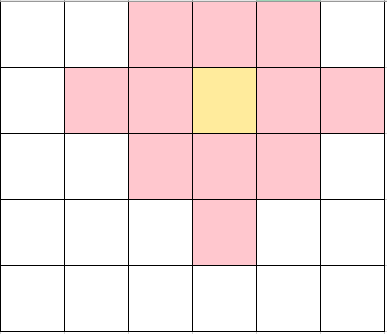
\includegraphics[width=.7\textwidth,height=.7\textheight,keepaspectratio]{images/dead_zone.PNG}
\end{figure}
\sethebrew

באיור 
\ref{fig: dead zone}
אפשר לראות שאם נלחץ על לחצן בצהוב האזור המת הי האזור באדום כולל 
הלחצן עצמו.
תכונה זה כלי מרכזי בהוכחה במשפט הבאה

\begin{theorem}
    \label{thrm: bigger then 7x7 board no minimal solution}
    במשחק על לוח 
    $m \times n$
    שמתקיים
    $\min(m,n) >= 7$
    למשחק אין פתרון מינמלי
\end{theorem}

נניח ויש לנו לוח דו ממדי שמתואר כך נקודת התחלה בכיוון למטה 
"קומת ראשונה"
והולך כלפי מעלה לאינסוף 
ואינסוף לצד ימין וצד שמאל.
נקרה לכל שורה אינסופית
קומה ונמספר אותם מאחת לאינסוף לכן קראנו לקומה נמוכה ביותר קומה ראשונה
נרצה למצוא פתרון מינמלי ללוח
וגישה לחיפוש הפתרון תהיה
להדליק שורה אחר שורה במלואה,
היות ושורת אינסופיות נציעה אסטרטגיה להדלקת השורה וניראה את הקשיים שנפגוש.
אם נרצה להדליק 
את כל קומה ראשנה רק על ידי לחצות 
בשורה ראשונה נקבל את הדפוס 
שאם לחצתי על לחצן מסוים חייב אני ללחוץ על לחצן
$3$
מימינו
כמו שמתואר באיור
\ref{fig: fill first stage only pressing first stage}
שמתאר לחצנים בירוק כלחצנים שנלחצו 
צהוב לחצנים שנדלקו ובאדום אזורים מתים שלא נדלקו.
באיור מוצג רק שתי לחיצות עוקבות של אסטרטגיה זה אבל כך נדליק את השורה הראשונה.

נשים לב באיור 
\ref{fig: fill first stage only pressing first stage}
על שני אזורים המתים הצמודים שלא נדלקו שצמודים אחד לשני כדי להדליק את שינהם
לא נוכל לעשות זאת ללא כיבוי לחצן שכבר נדלק.
זאת אומר שאסטרטגיה שכזאת
נפסלת עבור מילוי משחק שקומה שלו גדולה מ
$1$.

\begin{figure}[ht]
    \caption{מילוי קומה ראשונה על ידי לחיצות רק בקומה ראשונה}
    \label{fig: fill first stage only pressing first stage}
    \unsethebrew
    \centering
    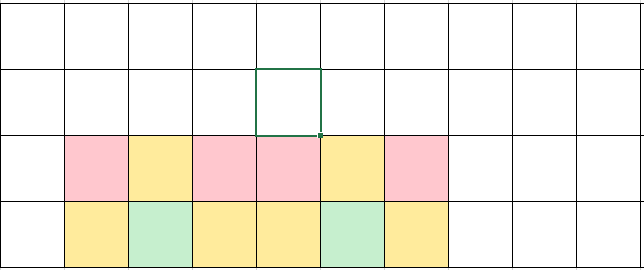
\includegraphics[width=.7\textwidth,height=.7\textheight,keepaspectratio]{images/first_stage_fill_only_first_stage_click.PNG}
\end{figure}
\sethebrew

אסטרטגיה אחרת ויחידה למילוי קומה ראשונה הינה להדליק 
פעם לחצן בקומה ראשנה 
ופעם לחצן בקומה שניה צמודים.
היות ורק שני קומות ראשונות משנות את מצב הלחצנים בקומה ראשונה ולא קיים דפוסים נוספים
אפשריים למילוי שורה ראשונה בעזרת שני שורות עלו לכן עלו הן כל אסטרטגיות למילוי קומה ראשונה.

\begin{figure}[ht]
    \caption{מילוי קומה ראשונה}
    \label{fig: fill first stage second attempt}
    \unsethebrew
    \centering
    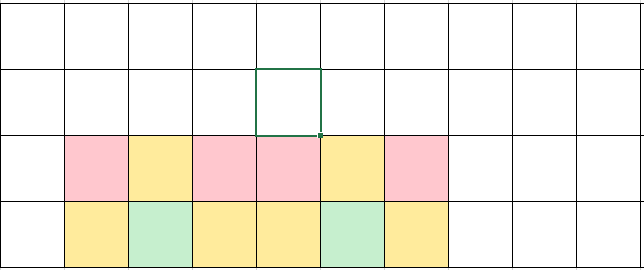
\includegraphics[width=.7\textwidth,height=.7\textheight,keepaspectratio]{images/first_stage_fill_only_first_stage_click.PNG}
\end{figure}
\sethebrew

באיור 
\ref{fig: fill first stage second attempt}
אפשר לראות הדגמה קטנה של אסטרטגיה שכזה.

נרצה להראות אסטרטגיה שכזה מובילה לאזורים מתים שלא ניתן למלאות 
כל עוד רוצים שהפתרון היה מינימלי.
אם נסתכל באיור 
\ref{fig: fill first stage second attempt fails}
ניראה שאזורים המתים ששלשת
המשבצות הרצופות באדום לא ניתן היה למלאה אותם לכן צירוף כזה אין חוקי
כלומר הראינו שלמשחק כפי שהגדרנו לא קיים בכלל פתרונות מינימליים.

\begin{figure}[ht]
    \caption{מילוי קומה ראשונה}
    \label{fig: fill first stage second attempt fails}
    \unsethebrew
    \centering
    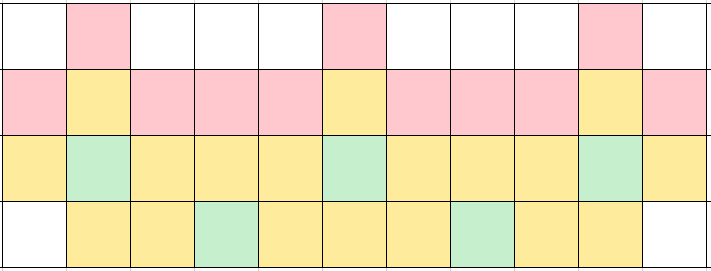
\includegraphics[width=.7\textwidth,height=.7\textheight,keepaspectratio]{images/first_stage_fill_only_first_stage_click_fail.PNG}
\end{figure}
\sethebrew

בשלב זה נרצה להקטין את הרוחב ואורך כך שאם קיים 
משחק אופטימלי בלוח המוקטן אסטרטגיות המילוי קומה קומה היחידות 
שהיו חוקיות הן עלו שהצגנו.
נדע שהקטנה לא היו לה פתרונות אופטימליים אם היו משבצות סמוכות באזורים מתים.

נחזור ונסתכל על איור 
\ref{fig: fill first stage only pressing first stage}
נשים לב שלכל לוח שמספר המשבצות לרוחב גדול או שווה 
מ
$6$
שיטת המילוי שכזה תהיה לא חוקית כי היו 
$2$
משבצות סמוכות שבאזורים לא חוקיים.
ובאיור 
\ref{fig: fill first stage second attempt fails}
ניראה
שלרוחב גדול או שווה 
מ
$5$
היות ובניה
של קומה ראשונה מסתמכת על זה שיש 
$7$
משבצות ניקח ליתר ביטחון 
$7$
משבצות ולכן באסטרטגיה זה לא היה פתרון מינמלי.

קיבלנו שאפשר להקטין את הלוח לרוחב של
$7$
משבצות 
ועדיין לא היה פתרון  מינמלי. 

את אותם טענות אפשר היה לבנות לא רק להגביל את רוחב ל
$7$
משבצות עלה גם לגובה.
לכן לסיכום קיבלנו 
במשחק על לוח 
שאורך או רוחב גדולים או שווים מ
$7$
אז
למשחק אין פתרון מינמלי
והוכחנו את הטענה.


\subsection{הלוח הגדול ביותר בעל פתרון מינמלי}
טענה 
\ref{thrm: bigger then 7x7 board no minimal solution} 
מגבילה מאד את המשחקים שיש להם פתרון מינמלי ובשיטת הפתרון שהצגנו
אחד המסקנות המתקבלות שאם יש שלוש קומות או יותר מתחילה
להיות בעיתיות בגישת מילוי השורות.
אפשר להבחין בתופעה זה היות וקיים פתרון מינמלי למשחק 
$2 \times m$
כאשר 
$m$
הוא אי זוגי
האסטרטגיה השנייה מאפשרת מילוי קומות ולקבל פתרון מינמלי
נדגים זאת על באיור 
\ref{fig: 2x9 have min sol}

\begin{figure}[ht]
    \caption{פתרון ללוח 
    $2 \times 9$}
    \label{fig: 2x9 have min sol}
    \unsethebrew
    \centering
    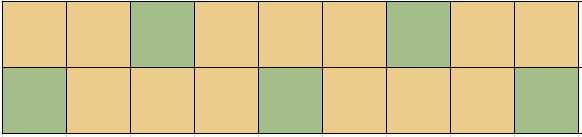
\includegraphics[width=.7\textwidth,height=.7\textheight,keepaspectratio]{images/2xm_sol.PNG}
\end{figure}
\sethebrew

לאחר שהבנו שלוחות בגודל 
$2 \times m$
כאשר 
$m$
אי זוגי 
קיים פתרון מינמלי נשאל מהו הלוח 
הגדול ביותר
בעל פתרון מינמלי כאשר 
הלוח אורך ורוחב גדולים מ
$2$.

לפי טענה 
\ref{thrm: bigger then 7x7 board no minimal solution} 
אין טעם לבדוק לוחות שעמודות ושורות גדולים מ
$7$
ומבניית ההוכחה 
אמרנו שאם 
הגדול של עמודות או שורות לא קטן
מ
$3$
כלומר נותר לבדוק לוחות שממד שלהם 
$m \times n$
שייכים לקבוצה
$\{ (m,n) : 2 < m,n <7 \}$.

אפשר לנסות ולחפש פתרון ידנית
או לעבור על כל הפתרונות של משחק רגיל ולבדוק עם יש מבניהם פתרון 
מינמלי.
נציעה דרך אחרת לחפש פתרון 
מינמלי
והיא בעזרת להשתמש באותה מטריצה שכנויות כפי שהגדרנו רק להגדיר 
את זה שהיא על חוג 
$\mathbb{Z}$.
בעזרת שימוש בחוג 
$\mathbb{Z}$
מאלצים את שפתרונות המתקבלים
שידליקו כל נורות אך ורק פעם אחת,
זאת מתקיים בעקבות 
משוואות האילוצים שהגדרנו ב
\ref{ def: depndeciy equation}
שמאלצות את הסכום להיות שווה לאחד
,
אם נסתכל על נוסחה של משוואת האילוצים הכללים 
נוסחה
\ref{eq: depndeciy equation}
היות וחיבור על השלמים לכן 
מאולצים במשוואה זה שהיה לחצן בודד לחוץ 
לכן פתרון מערכת המשוואות מתאר פתרון 
מינמלי של משחק.
התיאוריה שפיתחנו באלגברה לינארית הייתה תקפה לשדות 
אבל כלי תכנות שהשתמשנו
בעבודה זה יודע לפתור גם על חוג של השלמים 
והסמכנו על הכלי כדי לבדוק את המקרים
שממדים שייכם לקבוצה 
$\{ (m,n) : 2 < m,n <7 \}$
וקיבלנו שהלוח
היחיד בקבוצת הממדים העלו שיש לו פתרון מינמלי 
הוא
לוח 
$4 \times 4$
ופתרון מתואר באיור 
\ref{fig:4x4_have_min_sol}

\begin{figure}[ht]
    \caption{פתרון ללוח 
    $4 \times 4$}
    \label{fig:4x4_have_min_sol}
    \unsethebrew
    \centering
    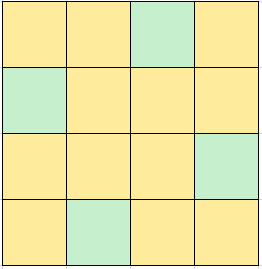
\includegraphics[width=.7\textwidth,height=.7\textheight,keepaspectratio]{images/4x4_min_sol.PNG}
\end{figure}
\sethebrew

\newpage
\section{נספחים}
מימוש של הפרויקט בוצע על ידי 
שפת תוכנה 
\L{Python}
עם הכלי 
\L{Sage}.

\unsethebrew
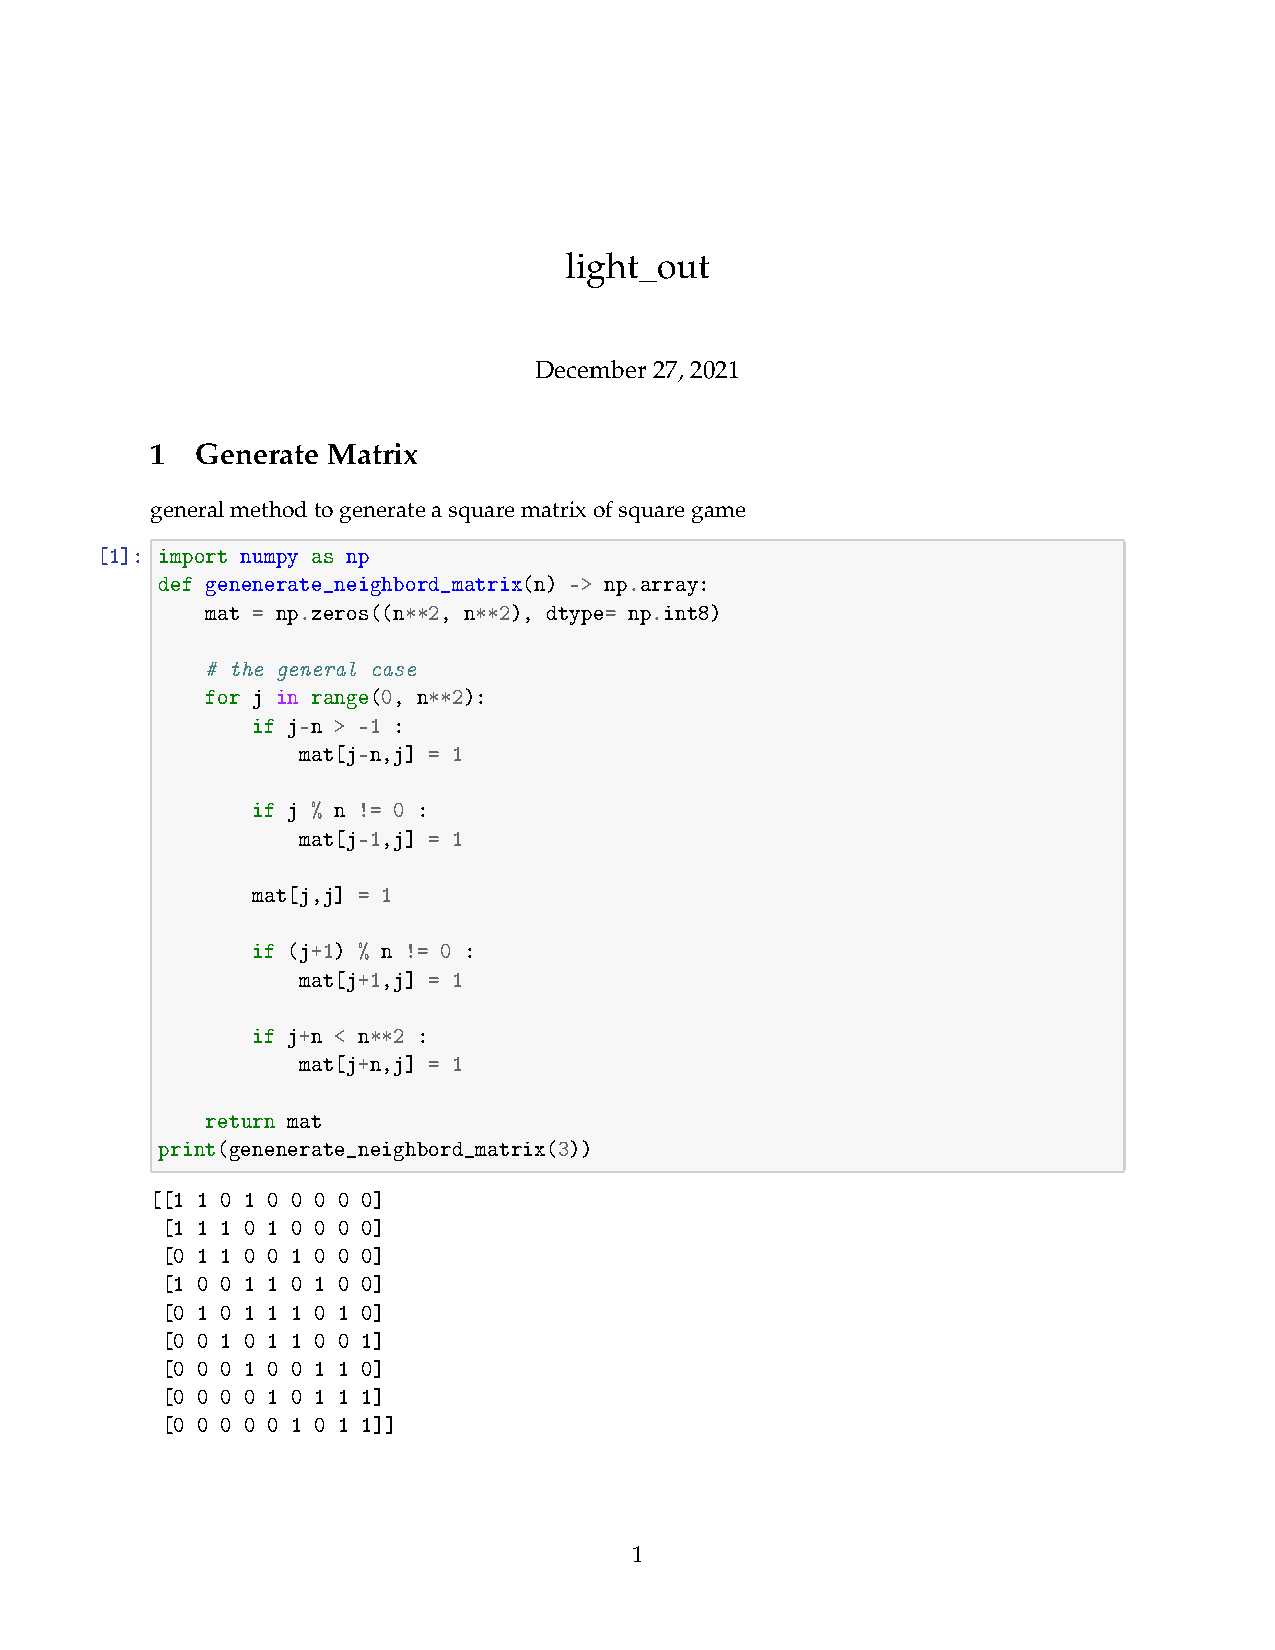
\includepdf[pages=-]{light_out_jupyter.pdf}
\sethebrew
%----------------------------------------------------------------------------------------
%   רשימת מקורות
%----------------------------------------------------------------------------------------
\newpage
\begin{thebibliography}{99}
\unsethebrew
\bibitem{B1} ALL LIGHTS AND LIGHTS OUT
An investigation among lights and shadows by
SUMA magazine’s article by Rafael Losada
Translated from Spanish by Ángeles Vallejo

\bibitem{B2} Lecture 24: Light out Puzzle , SFU faculty of scienc department of mathematics
\bibitem{B3} algebra book TODO: fill it
\end{thebibliography}

\end{document} 
